\documentclass[11pt,a4paper]{article}

% ------------------------------------------------------------------ packages
\usepackage[utf8]{inputenc}
\usepackage[T1]{fontenc}
\usepackage{lmodern}
\usepackage[a4paper,margin=2.2cm,headheight=14pt]{geometry}
\usepackage{graphicx}
\usepackage{amsmath,amssymb}
\usepackage{booktabs,tabularx,array,multirow}
\usepackage{xcolor}
\usepackage{fancyhdr}
\usepackage{titlesec}
\usepackage{caption,subcaption}
\usepackage{enumitem}
\usepackage{listings}
\usepackage[most]{tcolorbox}
\usepackage{wrapfig}
\usepackage{float}
\usepackage[hidelinks]{hyperref}

\graphicspath{{figures/}}

% ------------------------------------------------------------------ page style
\pagestyle{fancy}
\fancyhf{}
\fancyhead[L]{Project Report}
\fancyhead[R]{\thepage}
\renewcommand{\headrulewidth}{0.4pt}

\titleformat{\section}{\normalfont\LARGE\bfseries}{\thesection.}{0.4em}{}
\titleformat{\subsection}{\normalfont\Large\bfseries}{\thesubsection.}{0.4em}{}
\titleformat{\subsubsection}{\normalfont\normalsize\bfseries}{\thesubsubsection}{1em}{}
\titlespacing*{\section}{0pt}{0pt}{1.2em}
\setlength{\parskip}{0.6em}
\setlength{\parindent}{0pt}

% ------------------------------------------------------------------ code listings
\definecolor{codebg}{HTML}{0B0F14}
\definecolor{codekw}{HTML}{4FC3F7}
\definecolor{codecm}{HTML}{6A9955}
\definecolor{codestr}{HTML}{E5A15A}
\lstdefinestyle{dark}{
  language=Python,
  backgroundcolor=\color{codebg},
  basicstyle=\ttfamily\scriptsize\color{white},
  keywordstyle=\color{codekw},
  commentstyle=\color{codecm},
  stringstyle=\color{codestr},
  showstringspaces=false,
  columns=fullflexible,
  breaklines=true,
  upquote=true,
}
\newtcblisting{pycode}[1]{
  enhanced, colback=codebg, colframe=codebg, coltitle=white,
  title={\bfseries #1}, fonttitle=\small, arc=0pt, boxrule=0pt,
  left=6pt, right=6pt, top=4pt, bottom=4pt,
  listing only, listing options={style=dark},
}
\newtcolorbox{console}{
  enhanced, colback=black!85, colframe=black, arc=1pt, boxrule=0pt,
  fontupper=\ttfamily\scriptsize\color{green!70!white}, left=6pt, right=6pt,
}

\newcommand{\MetalN}{77,432}
\newcommand{\MetalPos}{47.7}
\newcommand{\MagN}{64,410}
\newcommand{\MagPos}{20.6}
\newcommand{\StabN}{436,791}
\newcommand{\StabPos}{29.5}
\newcommand{\GapN}{78,164}
\newcommand{\GapPos}{6.7}
\newcommand{\MetalInBestMethod}{?}
\newcommand{\MetalInBestConfig}{?}
\newcommand{\MetalInBestComp}{?}
\newcommand{\MetalInBaseComp}{?}
\newcommand{\MetalInBaseConfig}{?}
\newcommand{\MetalInImpr}{?}
\newcommand{\MetalInFullComp}{?}
\newcommand{\MetalInDepComp}{?}
\newcommand{\MetalInDepAUC}{?}
\newcommand{\MetalInDepFone}{?}
\newcommand{\MetalInBestSSL}{?}
\newcommand{\MetalInBestSSLComp}{?}
\newcommand{\MetalGnBestMethod}{?}
\newcommand{\MetalGnBestConfig}{?}
\newcommand{\MetalGnBestComp}{?}
\newcommand{\MetalGnBaseComp}{?}
\newcommand{\MetalGnBaseConfig}{?}
\newcommand{\MetalGnImpr}{?}
\newcommand{\MetalGnFullComp}{?}
\newcommand{\MetalGnDepComp}{?}
\newcommand{\MetalGnDepAUC}{?}
\newcommand{\MetalGnDepFone}{?}
\newcommand{\MetalGnBestSSL}{?}
\newcommand{\MetalGnBestSSLComp}{?}
\newcommand{\MagInBestMethod}{?}
\newcommand{\MagInBestConfig}{?}
\newcommand{\MagInBestComp}{?}
\newcommand{\MagInBaseComp}{?}
\newcommand{\MagInBaseConfig}{?}
\newcommand{\MagInImpr}{?}
\newcommand{\MagInFullComp}{?}
\newcommand{\MagInDepComp}{?}
\newcommand{\MagInDepAUC}{?}
\newcommand{\MagInDepFone}{?}
\newcommand{\MagInBestSSL}{?}
\newcommand{\MagInBestSSLComp}{?}
\newcommand{\MagGnBestMethod}{?}
\newcommand{\MagGnBestConfig}{?}
\newcommand{\MagGnBestComp}{?}
\newcommand{\MagGnBaseComp}{?}
\newcommand{\MagGnBaseConfig}{?}
\newcommand{\MagGnImpr}{?}
\newcommand{\MagGnFullComp}{?}
\newcommand{\MagGnDepComp}{?}
\newcommand{\MagGnDepAUC}{?}
\newcommand{\MagGnDepFone}{?}
\newcommand{\MagGnBestSSL}{?}
\newcommand{\MagGnBestSSLComp}{?}
\newcommand{\StabInBestMethod}{?}
\newcommand{\StabInBestConfig}{?}
\newcommand{\StabInBestComp}{?}
\newcommand{\StabInBaseComp}{?}
\newcommand{\StabInBaseConfig}{?}
\newcommand{\StabInImpr}{?}
\newcommand{\StabInFullComp}{?}
\newcommand{\StabInDepComp}{?}
\newcommand{\StabInDepAUC}{?}
\newcommand{\StabInDepFone}{?}
\newcommand{\StabInBestSSL}{?}
\newcommand{\StabInBestSSLComp}{?}
\newcommand{\StabGnBestMethod}{?}
\newcommand{\StabGnBestConfig}{?}
\newcommand{\StabGnBestComp}{?}
\newcommand{\StabGnBaseComp}{?}
\newcommand{\StabGnBaseConfig}{?}
\newcommand{\StabGnImpr}{?}
\newcommand{\StabGnFullComp}{?}
\newcommand{\StabGnDepComp}{?}
\newcommand{\StabGnDepAUC}{?}
\newcommand{\StabGnDepFone}{?}
\newcommand{\StabGnBestSSL}{?}
\newcommand{\StabGnBestSSLComp}{?}
\newcommand{\KBest}{3}
\newcommand{\PCAVarTwo}{30.4}
\newcommand{\RulesStab}{67}
\newcommand{\RulesMag}{26}
\newcommand{\RulesMetal}{47}
\newcommand{\RulesGap}{6}
\newcommand{\AERtwo}{0.912}
\newcommand{\AERtwoMasked}{0.907}


% include a figure if it exists, otherwise a placeholder box (results still running)
\newcommand{\safeimg}[2]{\IfFileExists{figures/#2}{\includegraphics[width=#1]{#2}}{%
  \fbox{\parbox[c][3cm][c]{#1}{\centering\small pending: \texttt{\detokenize{#2}}}}}}
% input a generated table if it exists (an experiment may still be running)
\newcommand{\maybeinput}[1]{\IfFileExists{generated/#1.tex}{\input{generated/#1}}{%
  \begin{center}\fbox{\small pending: \texttt{\detokenize{#1}}}\end{center}}}
% one figure with optional second panel
\newcommand{\resfig}[3]{\begin{figure}[H]\centering\safeimg{#1}{#2}\caption{#3}\end{figure}}

\begin{document}

% ================================================================== title page
\begin{titlepage}
  \centering
  \begin{minipage}{0.48\textwidth}
    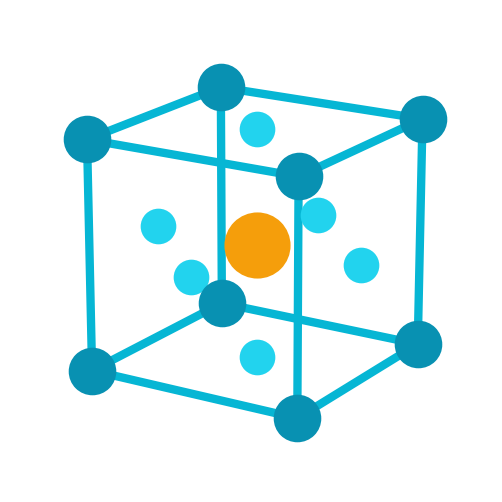
\includegraphics[height=2.7cm]{logos/crystal.png}
  \end{minipage}\hfill
  \begin{minipage}{0.48\textwidth}\raggedleft
    
\includegraphics[height=2.7cm]{logos/esi.png}
  \end{minipage}

  \vspace{1.4cm}
  \rule{\textwidth}{0.4pt}\\[0.6cm]
  {\fontsize{36}{40}\selectfont\bfseries Project Report}\\[0.5cm]
  \rule{\textwidth}{0.4pt}

  \vspace{1.6cm}
  {\Large\bfseries Theme: Materials Discovery and Property Prediction\\(MI--SSL)}

  \vspace{1.8cm}
  \begin{minipage}{0.78\textwidth}\centering\large
    This project addresses the critical problem of labeled data scarcity in materials
    science by using Semi-Supervised Learning (SSL) techniques to predict the stability,
    magnetism, metallicity and band gap of inorganic materials.
  \end{minipage}

  \vspace{2cm}
  {\large\bfseries Group Members:}\\[0.4cm]
  \large Laref Ibrahim\\[0.15cm]
  Nemouchi Faycal Abdelhadi\\[0.15cm]
  Zerradi Abdelbasset\\[0.15cm]
  Medelci Djezzar Aymen

  \vfill
  {\small\bfseries \today}
\end{titlepage}

\tableofcontents
\clearpage
\listoffigures
\clearpage

\clearpage
\section{Introduction and Problem Statement}

\subsection{The Challenge: Stability and Functionality}

Materials discovery is a high-stakes filtration process: hundreds of thousands of candidate
compositions are screened to identify the few that can actually be synthesized and that have
the property an application needs. Early success in this pipeline hinges on overcoming two
critical challenges:

\begin{itemize}
  \item \textbf{Predicting Stability:} a material must be thermodynamically stable (on or near
  the convex hull of formation energies) to be made in the laboratory. Compositions resembling
  known stable compounds are statistically more likely to succeed, offering an early signal of
  viability.
  \item \textbf{Predicting Functionality:} electronic and magnetic behaviour (metal or
  insulator, magnetic or not, band gap inside the photovoltaic window) decides whether a
  material is useful for batteries, magnets, electronics or solar cells. Detecting these
  properties early avoids costly quantum-mechanical simulations and failed syntheses, saving
  both time and resources.
\end{itemize}

The essential question is clear: \emph{``Is this composition stable enough to be made, and does
it have the property we are looking for?''}

\subsection{The Data Dilemma}

Applying AI to this challenge is difficult due to an imbalance in available data:

\begin{enumerate}
  \item \textbf{Labeled Data is Scarce:} a reliable property label requires a density
  functional theory (DFT) calculation, costing hours to days of computing per material, or an
  even more expensive laboratory measurement. Consequently, high-quality labeled datasets
  remain limited compared with the space of possible compositions.
  \item \textbf{Unlabeled Data is Abundant:} high-throughput and generative searches such as
  Google DeepMind's GNoME propose hundreds of thousands of new compositions, most of which lack
  the property we want to predict.
\end{enumerate}

This raises a crucial question:

\begin{center}
\textbf{How can we harness the vast sea of unlabeled compositions to improve property
predictions, even when high-quality labeled data is scarce?}
\end{center}

Our solution is \textbf{Semi-Supervised Learning (SSL)}, which bridges the gap between scarce
labels and abundant unlabeled data. By leveraging unlabeled compositions intelligently, SSL aims
to enhance model performance and deliver more accurate and reliable property predictions.

\subsection{Complementary Approaches: SSL and Traditional Materials Informatics}

In addition to Semi-Supervised Learning, we implemented a traditional materials-informatics
pipeline for \textbf{photovoltaic band-gap classification}. This classical approach emphasizes
interpretability, descriptor optimization via genetic algorithms, and an OECD-style
applicability-domain assessment. We complete the study with \textbf{unsupervised learning}
(association-rule mining and clustering) and \textbf{self-supervised pre-training} on the
unlabeled pool. Together, these approaches provide complementary strategies: SSL leverages
unlabeled data for general property endpoints, unsupervised learning reveals the hidden
chemical structure of the data, and the traditional pipeline offers explainable, optimized
models for a well-characterized endpoint.

\clearpage
\section{Materials Informatics and Compositional Similarity}

Materials informatics (MI), and in particular Quantitative Structure--Property Relationship
(QSPR) modeling, is a key tool in modern materials discovery. Its main idea is simple:
\textbf{materials with similar compositions and chemistry often have similar physical
properties}. This directly relates to our challenge of predicting whether a material is
stable, magnetic or metallic using limited computed data (Section~1).

MI represents every material as a numerical vector called a \textbf{descriptor} vector. For a
chemical formula, the most widely used descriptors are the \emph{Magpie} statistics: for 22
elemental properties (electronegativity, covalent radius, number of valence electrons,
melting temperature, elemental band gap, magnetic moment, \dots) we compute the
composition-weighted minimum, maximum, range, mean, average deviation and mode. Models trained
on materials with known properties can then predict the properties of new compositions in
milliseconds, which is particularly useful when labeled data is scarce and the pool of
untested candidates is huge.

A typical MI workflow includes:

\begin{enumerate}
  \item Collecting a dataset of materials with known properties.
  \item Calculating composition (or structure) descriptors.
  \item Selecting the most relevant descriptors to avoid overfitting.
  \item Building predictive models using regression or classification methods.
  \item Validating models with cross-validation and external test sets.
\end{enumerate}

MI not only predicts properties but also highlights which chemical features matter, guiding
the design of better materials. It also reduces reliance on expensive DFT calculations and
laboratory synthesis.

\begin{figure}[H]
  \centering
  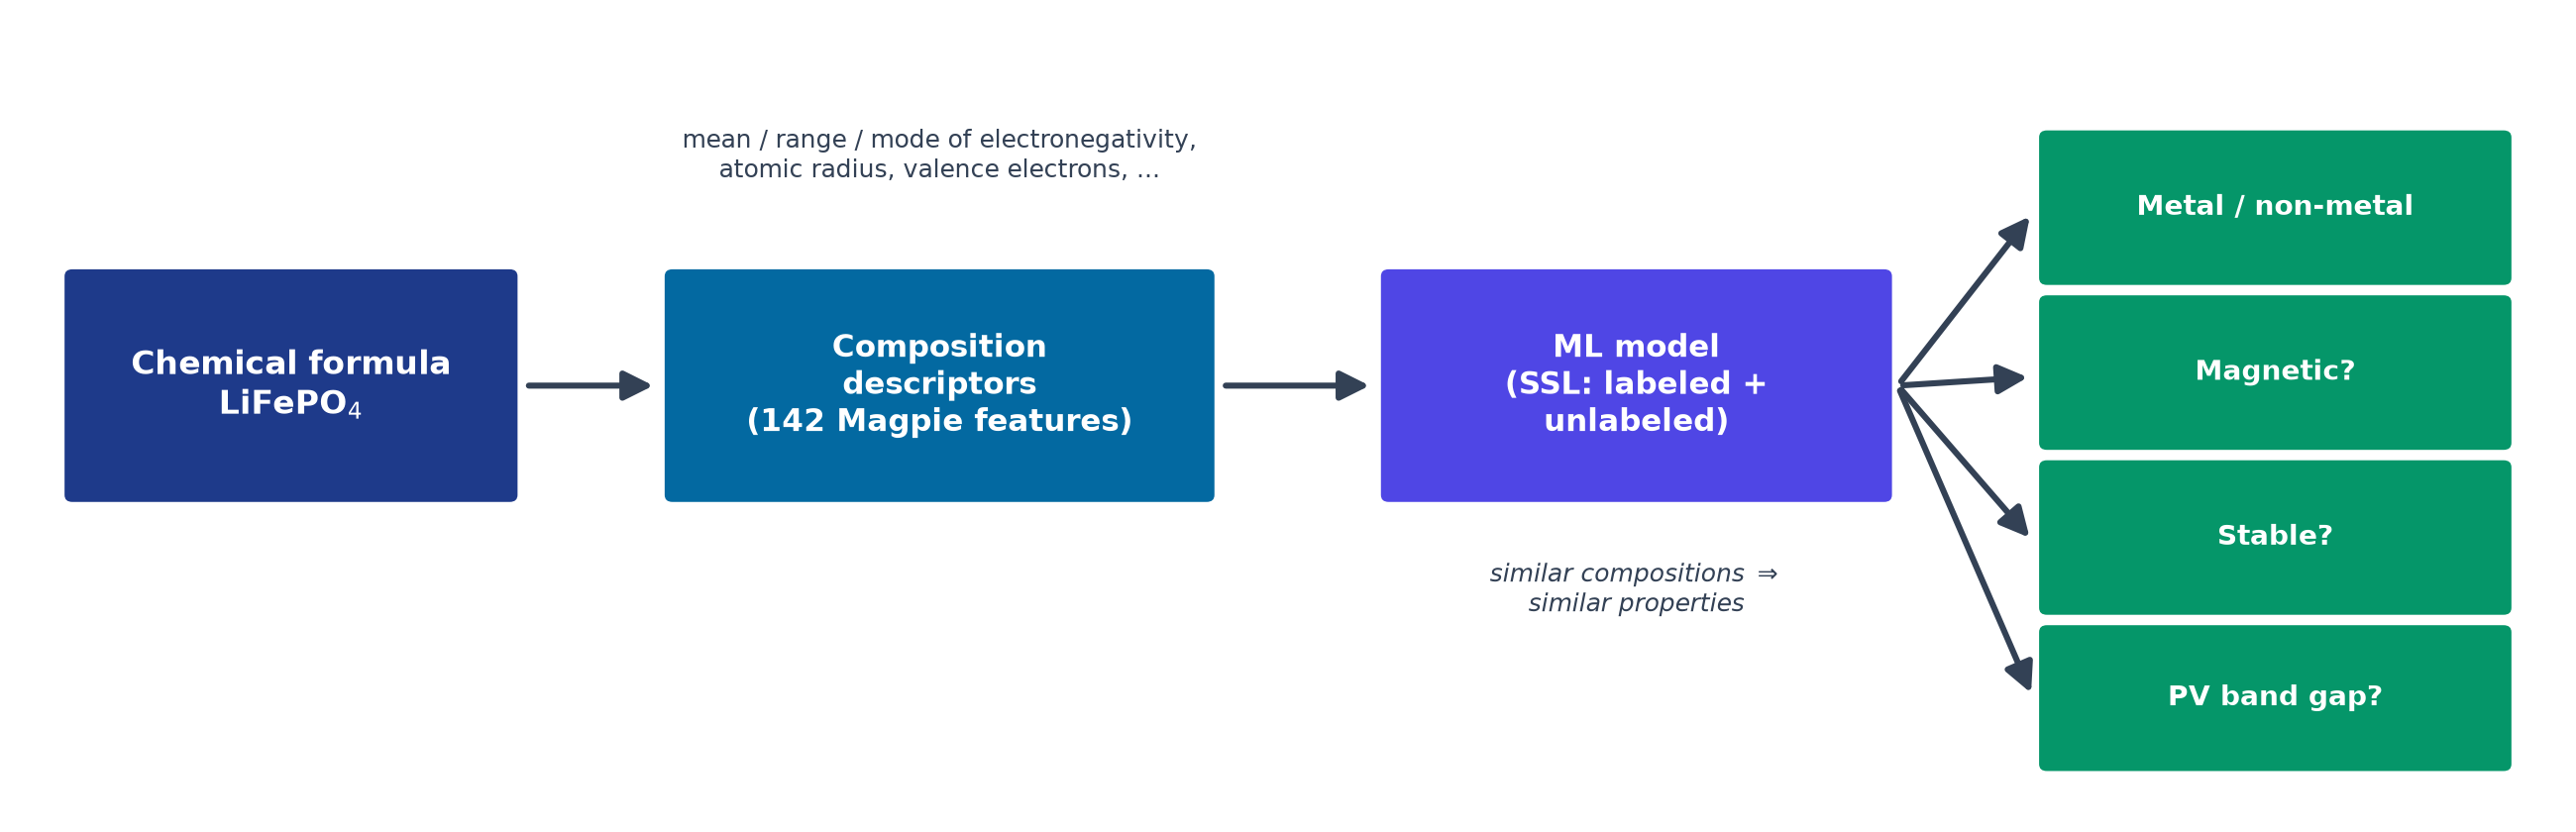
\includegraphics[width=\textwidth]{schematics/mi_principle.png}
  \caption{Materials-informatics principle}
\end{figure}

Building on MI, Semi-Supervised Learning (SSL) can further improve predictions by
incorporating the large pool of unlabeled compositions. Combining MI with SSL allows models to
learn from both labeled and unlabeled data, addressing the challenges of property prediction
and data scarcity.

\clearpage
\section{Semi-Supervised Learning as a Solution}

Semi-Supervised Learning (SSL) lies between supervised and unsupervised learning. Its main goal
is to leverage a small labeled dataset along with a large pool of unlabeled data to improve
model generalization, especially when acquiring labels is expensive or time-consuming. This
makes SSL particularly relevant for materials discovery, where every label costs a DFT
calculation or an experiment (Section~1).

In this project, we explore five SSL algorithms. The wrapper methods are built on
\textbf{tree-ensemble classifiers}: Random Forest as the reference learner (as in classical
QSAR/QSPR studies) and a LightGBM gradient-boosting learner tuned with Optuna:

\begin{itemize}
  \item \textbf{Self-Learning (Pseudo-Labeling):} a tree-ensemble model is trained on labeled
  data, then used to predict labels for unlabeled data. High-confidence predictions are added
  iteratively to the training set to refine the model.
  \item \textbf{Co-Training (Multi-View Learning):} two models are trained on different
  feature subsets (views) of the same data: elemental-property statistics and
  stoichiometry/valence-electron descriptors. Each model labels unlabeled data for the other,
  exploiting complementary information.
  \item \textbf{Label Propagation:} models the dataset as a graph where nodes are materials and
  edges represent compositional similarity. Labels propagate from labeled to unlabeled nodes,
  respecting the data manifold.
  \item \textbf{Label Spreading:} similar to label propagation, but includes a normalization
  step to ensure a smooth label distribution across the graph and to reduce sensitivity to
  noisy edges.
  \item \textbf{Cluster-then-Label:} an unsupervised K-Means clustering of labeled and
  unlabeled materials; unlabeled members of label-pure clusters receive the cluster's label
  (the \emph{cluster assumption} of SSL).
\end{itemize}

\begin{table}[H]
\centering\small
\renewcommand{\arraystretch}{1.25}
\begin{tabularx}{\textwidth}{>{\bfseries}l X X X X X}
\toprule
Feature & Self-Learning & Co-Training & Label Propagation & Label Spreading & Cluster-then-Label\\
\midrule
Approach & Iterative pseudo-labeling & Multi-view learning & Graph-based, hard labels &
Graph-based, soft labels & Clustering + label transfer\\
Strengths & Simple, easy to implement, scalable & Exploits complementary features, reduces bias
& Captures manifold structure, smooth predictions & Smooths labels, robust to noise & Very fast,
uses global structure of the pool\\
Limitations & Sensitive to initial model errors & Requires distinct views, can be complex &
Computationally intensive, sensitive to graph quality & Same as label propagation, can
over-smooth & Fails when clusters mix classes\\
\bottomrule
\end{tabularx}
\end{table}

By comparing these SSL methods on our materials datasets, we aim to identify which technique
best balances prediction accuracy and robustness when labeled data is limited.

\clearpage
\section{Preprocessing}

The preprocessing pipeline transforms raw materials databases (chemical formulas, crystal
structures and computed properties) into structured, numerical datasets suitable for
Semi-Supervised Learning. This process is implemented in two stages for each dataset:
\textbf{Data Enhancement} (label definition and descriptor engineering) and
\textbf{EDA/Processing} (exploration, outlier handling, normalization and splitting).

\subsection{Dataset Overview}

We utilize three large, open, widely cited databases to address the twin challenges of
\textbf{Stability} and \textbf{Functionality}, plus the GNoME database as the unlabeled pool.
Every database is reduced to \emph{one row per unique composition} (reduced formula), which
removes duplicated polymorphs and prevents leakage between training and test sets.

\subsubsection{1. Metallicity (Materials Project)}
Focused on the \textbf{electronic-behaviour challenge}, this dataset distinguishes metals from
semiconductors and insulators.
\begin{itemize}
  \item \textbf{Source:} Materials Project, through the Matbench benchmark
  \texttt{matbench\_mp\_is\_metal} (106,113 DFT entries).
  \item \textbf{Size:} \MetalN{} unique compositions (\MetalPos{}\% metals).
  \item \textbf{Target Variable:} \texttt{is\_metal} (Binary: 1 = metal, 0 = non-metal;
  polymorphs aggregated by majority vote).
  \item \textbf{Goal:} predict whether a composition conducts like a metal or has a band gap.
\end{itemize}

\subsubsection{2. Magnetism (JARVIS-DFT)}
Focused on the \textbf{functional-property challenge} for magnetic and spintronic materials.
\begin{itemize}
  \item \textbf{Source:} JARVIS-DFT 3D database (NIST), 93,902 DFT calculations.
  \item \textbf{Size:} \MagN{} unique compositions (\MagPos{}\% magnetic).
  \item \textbf{Target Variable:} \texttt{is\_magnetic} (Binary: 1 if the total magnetic moment
  of the lowest-energy polymorph is at least $0.5\,\mu_B$).
  \item \textbf{Goal:} identify magnetic compositions.
\end{itemize}

\subsubsection{3. Thermodynamic Stability (Alexandria)}
Focused on the \textbf{synthesizability challenge} over a very broad chemical space.
\begin{itemize}
  \item \textbf{Source:} Alexandria PBE 3D database (ICAMS, Ruhr-Universit\"at Bochum), release
  2025.07.02; five chunks = 500,000 DFT calculations.
  \item \textbf{Size:} \StabN{} unique compositions (\StabPos{}\% stable).
  \item \textbf{Target Variable:} \texttt{is\_stable} (Binary: 1 if the lowest-energy polymorph
  lies at most 0.05\,eV/atom above the convex hull).
  \item \textbf{Goal:} validate the models' ability to generalize to a very large and diverse
  chemical space.
\end{itemize}

\textbf{Unlabeled pool (GNoME).} The 554,054 compositions of the GNoME stable-materials summary
(Google DeepMind, 2023) are used as \emph{unlabeled} data; any composition already present in a
labeled dataset is removed from the pool. A second, classical SSL setting is also studied in
which the unlabeled pool consists of the remaining training compositions of the same database
with their labels hidden.

\begin{table}[H]
\centering\small
\begin{tabular}{llrrr}
\toprule
Dataset & Source & Raw entries & Unique compositions & Positive rate\\
\midrule
Metallicity & Materials Project & 106,113 & \MetalN{} & \MetalPos{}\%\\
Magnetism & JARVIS-DFT & 93,902 & \MagN{} & \MagPos{}\%\\
Stability & Alexandria & 500,000 & \StabN{} & \StabPos{}\%\\
PV band gap (Sec.~5.5) & Materials Project & 106,113 & \GapN{} & \GapPos{}\%\\
Unlabeled pool & GNoME & 554,054 & 554,054 & --\\
\bottomrule
\end{tabular}
\caption*{Datasets used in this project (all open, no API key required).}
\end{table}

\clearpage
\subsection{Preprocessing Workflow}

The following steps are applied consistently across all datasets using the
\texttt{data\_enhancing} and \texttt{eda} notebooks.

\begin{enumerate}[leftmargin=*]
\item \textbf{Feature Engineering (matminer/Magpie):} we convert raw chemical formulas into a
comprehensive set of 142 composition descriptors: 132 Magpie statistics of 22 elemental
properties (electronegativity, covalent radius, valence electrons, melting temperature,
elemental band gap and magnetic moment, \dots), 6 stoichiometric $p$-norms and 4
valence-orbital fractions. Because matminer featurizes one composition at a time, we
re-implemented the same statistics in vectorized NumPy form; the result is identical to
matminer (maximum absolute difference $2\times10^{-13}$) and featurizes 240,000 compositions in
3.6\,s, which makes the 1.1 million compositions of this project tractable.

\begin{figure}[H]
\begin{pycode}{Composition featurization (pipeline/featurize.py)}
from featurize import featurize_formulas
import pandas as pd

formulas = pd.Series(["LiFePO4", "Fe2O3", "GaAs", "Nd2Fe14B", "SrTiO3"])
X, ok = featurize_formulas(formulas)          # 142 descriptors per composition
# mean / avg_dev / min / max / range / mode of 22 elemental properties,
# computed with sparse fraction matrices:  mean = F @ P
print(X.shape)                                # (5, 142)
\end{pycode}
\caption{Extraction of composition descriptors with the Magpie featurizer.}
\end{figure}

\begin{figure}[H]
  \centering
  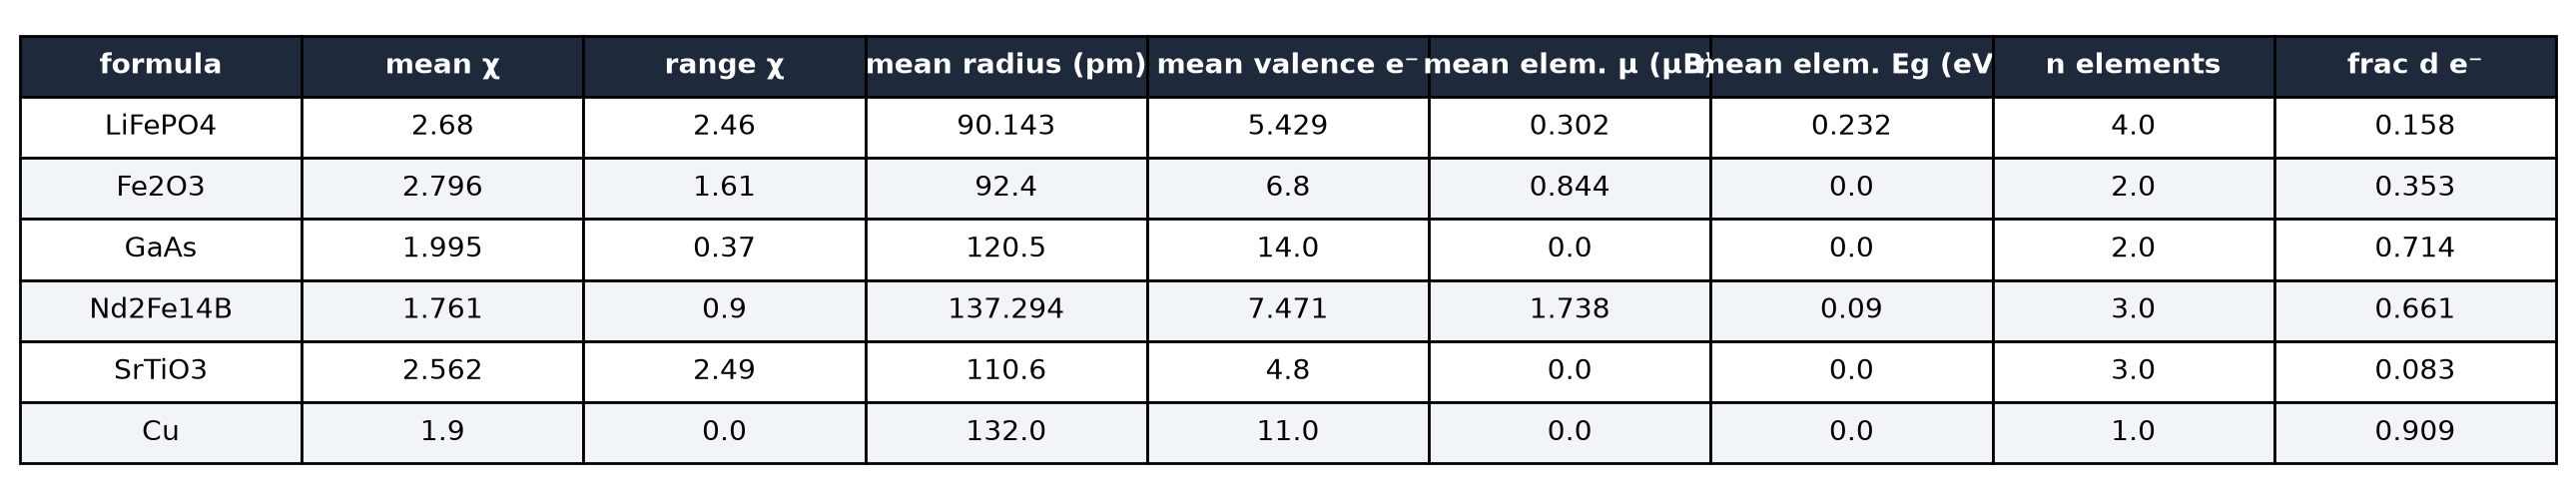
\includegraphics[width=\textwidth]{schematics/descriptor_examples.png}
  \caption{Extraction of physicochemical descriptors for example compositions.}
\end{figure}

\item \textbf{Exploring our Data:} before training, we analyzed every labeled dataset to
understand how the descriptors interact with each other and with the target variable. We
generated correlation heatmaps to identify strong associations between physicochemical
properties (such as electronegativity or valence-electron count) and the
stability/magnetism/metallicity labels. This step was crucial to verify that our engineered
features carry meaningful signals for classification. Figures~\ref{fig:corr}--\ref{fig:outliers}
show the Alexandria stability dataset (the largest one); the notebooks contain the same
analysis for every dataset.

\begin{figure}[H]
  \centering
  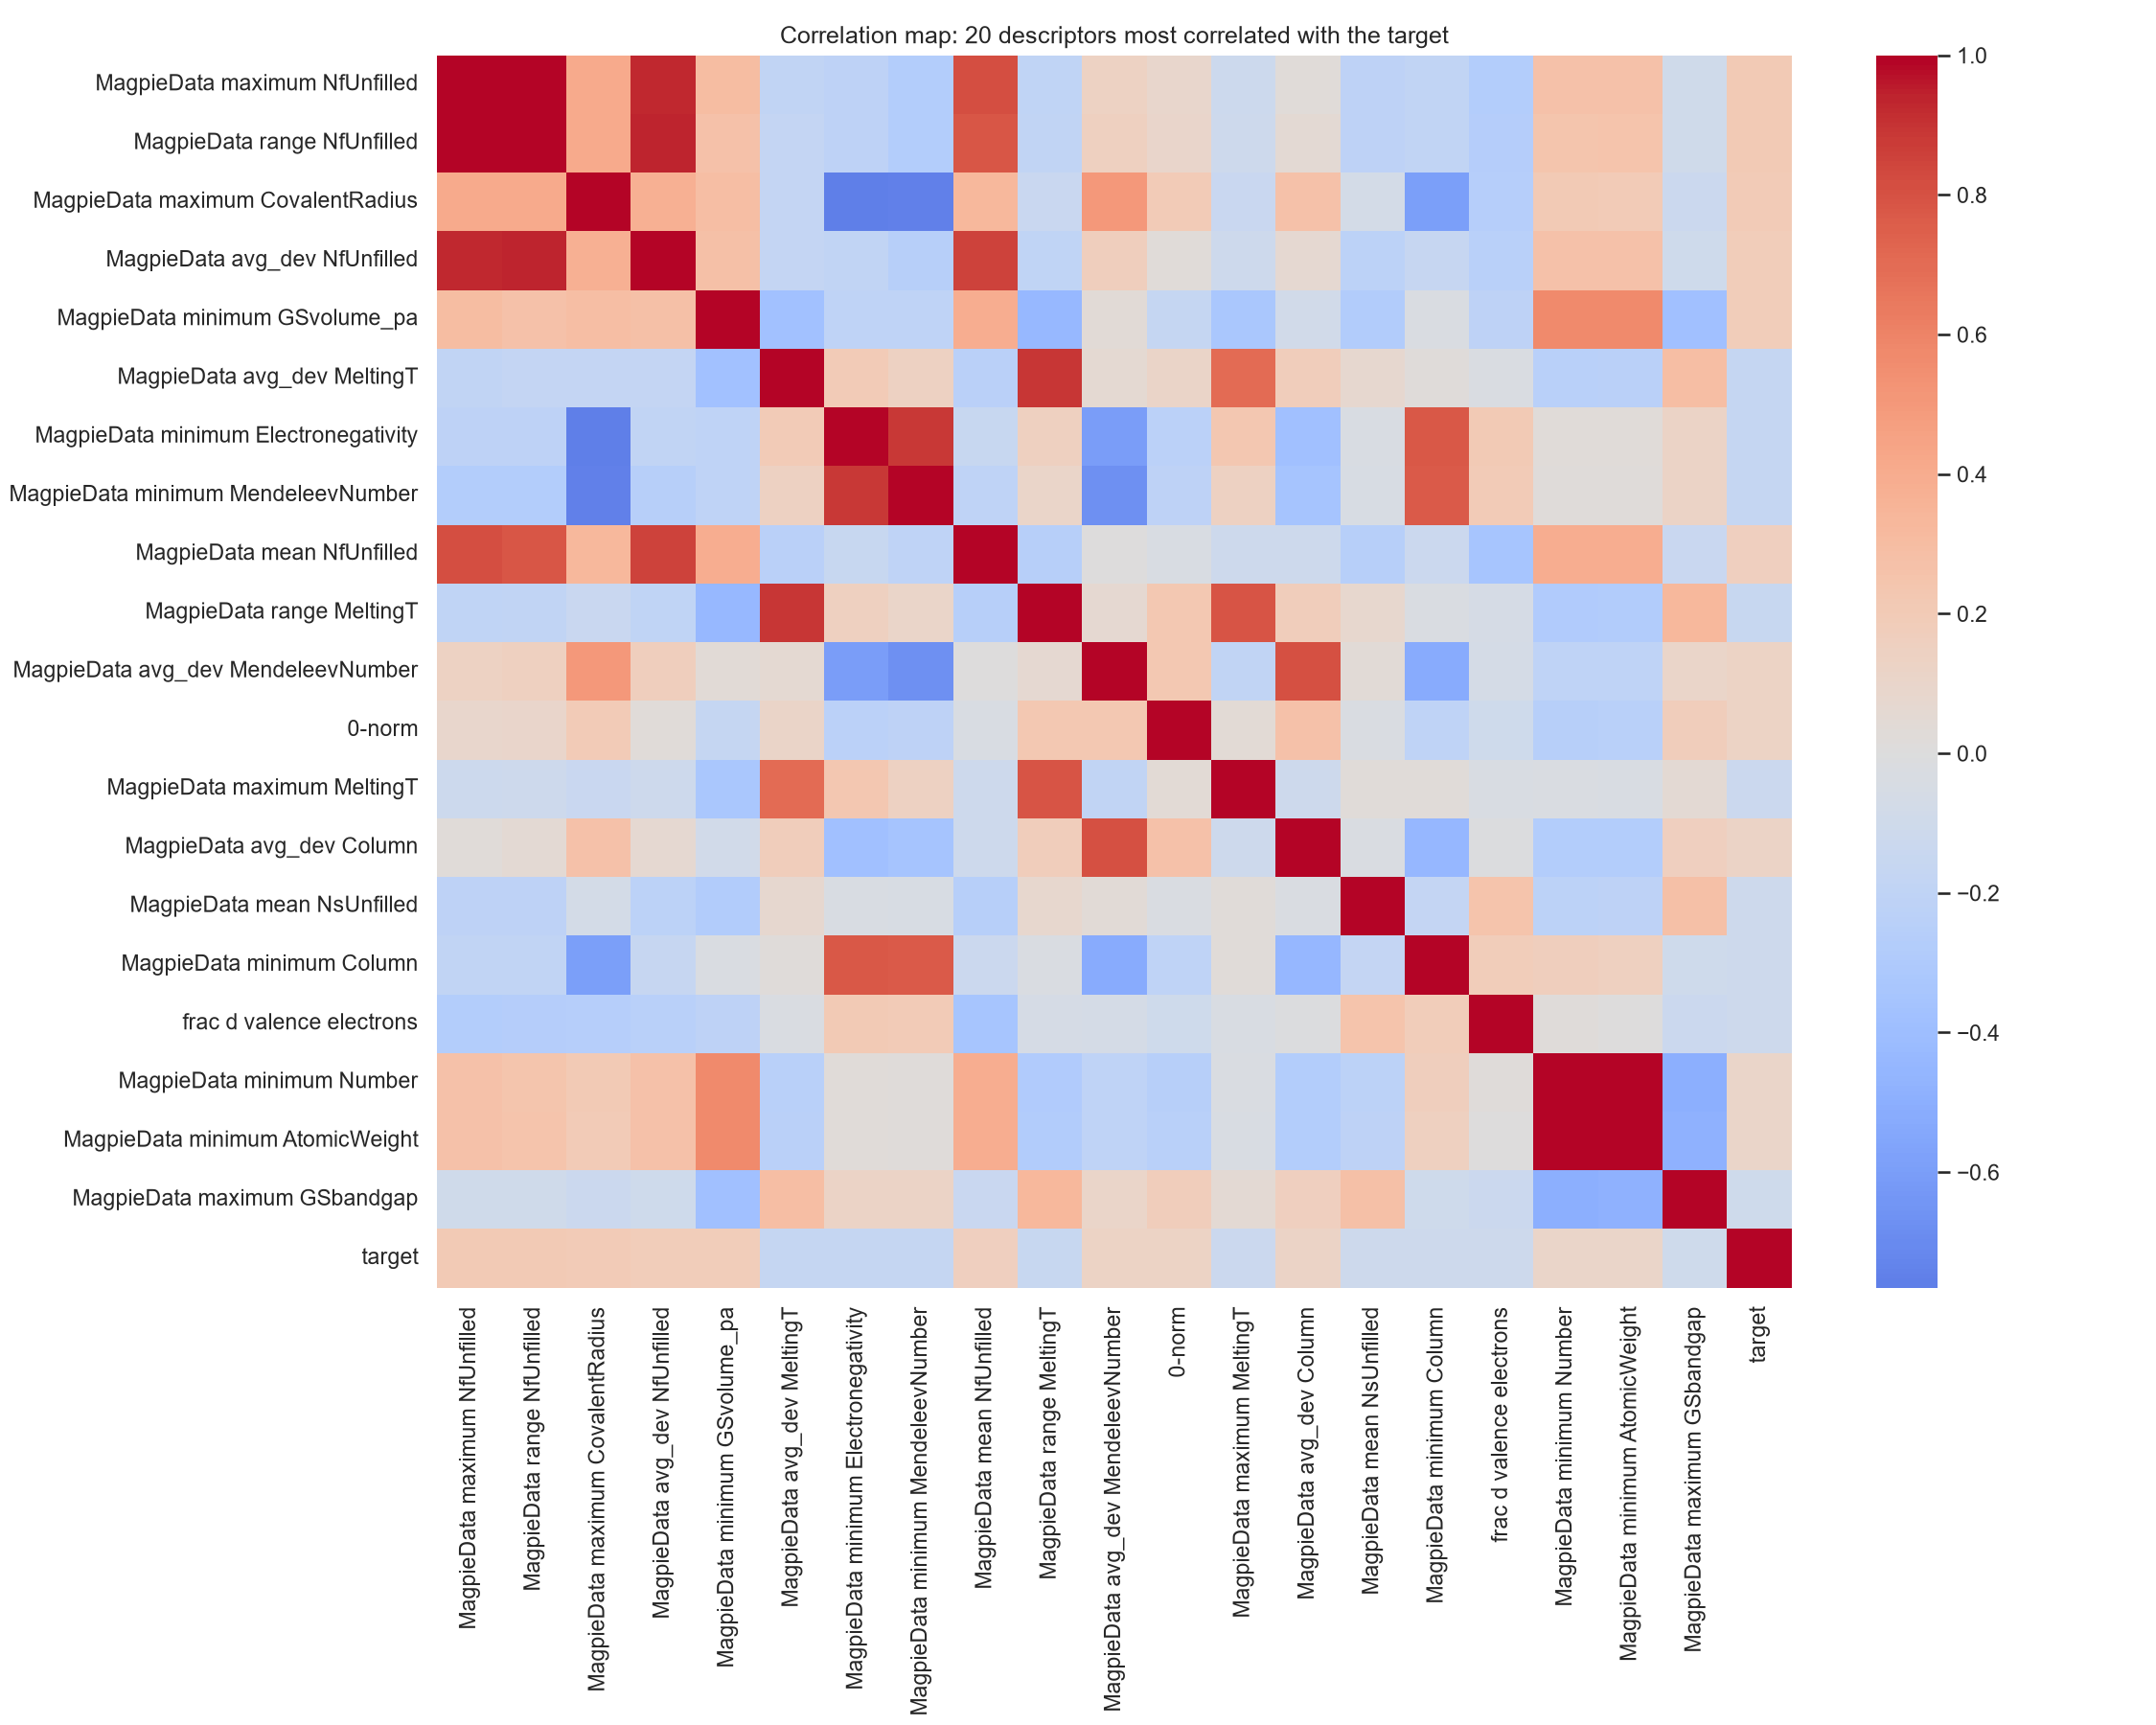
\includegraphics[width=0.82\textwidth]{stability/correlation_map.png}
  \caption{Correlation Map}\label{fig:corr}
\end{figure}

\begin{figure}[H]
  \centering
  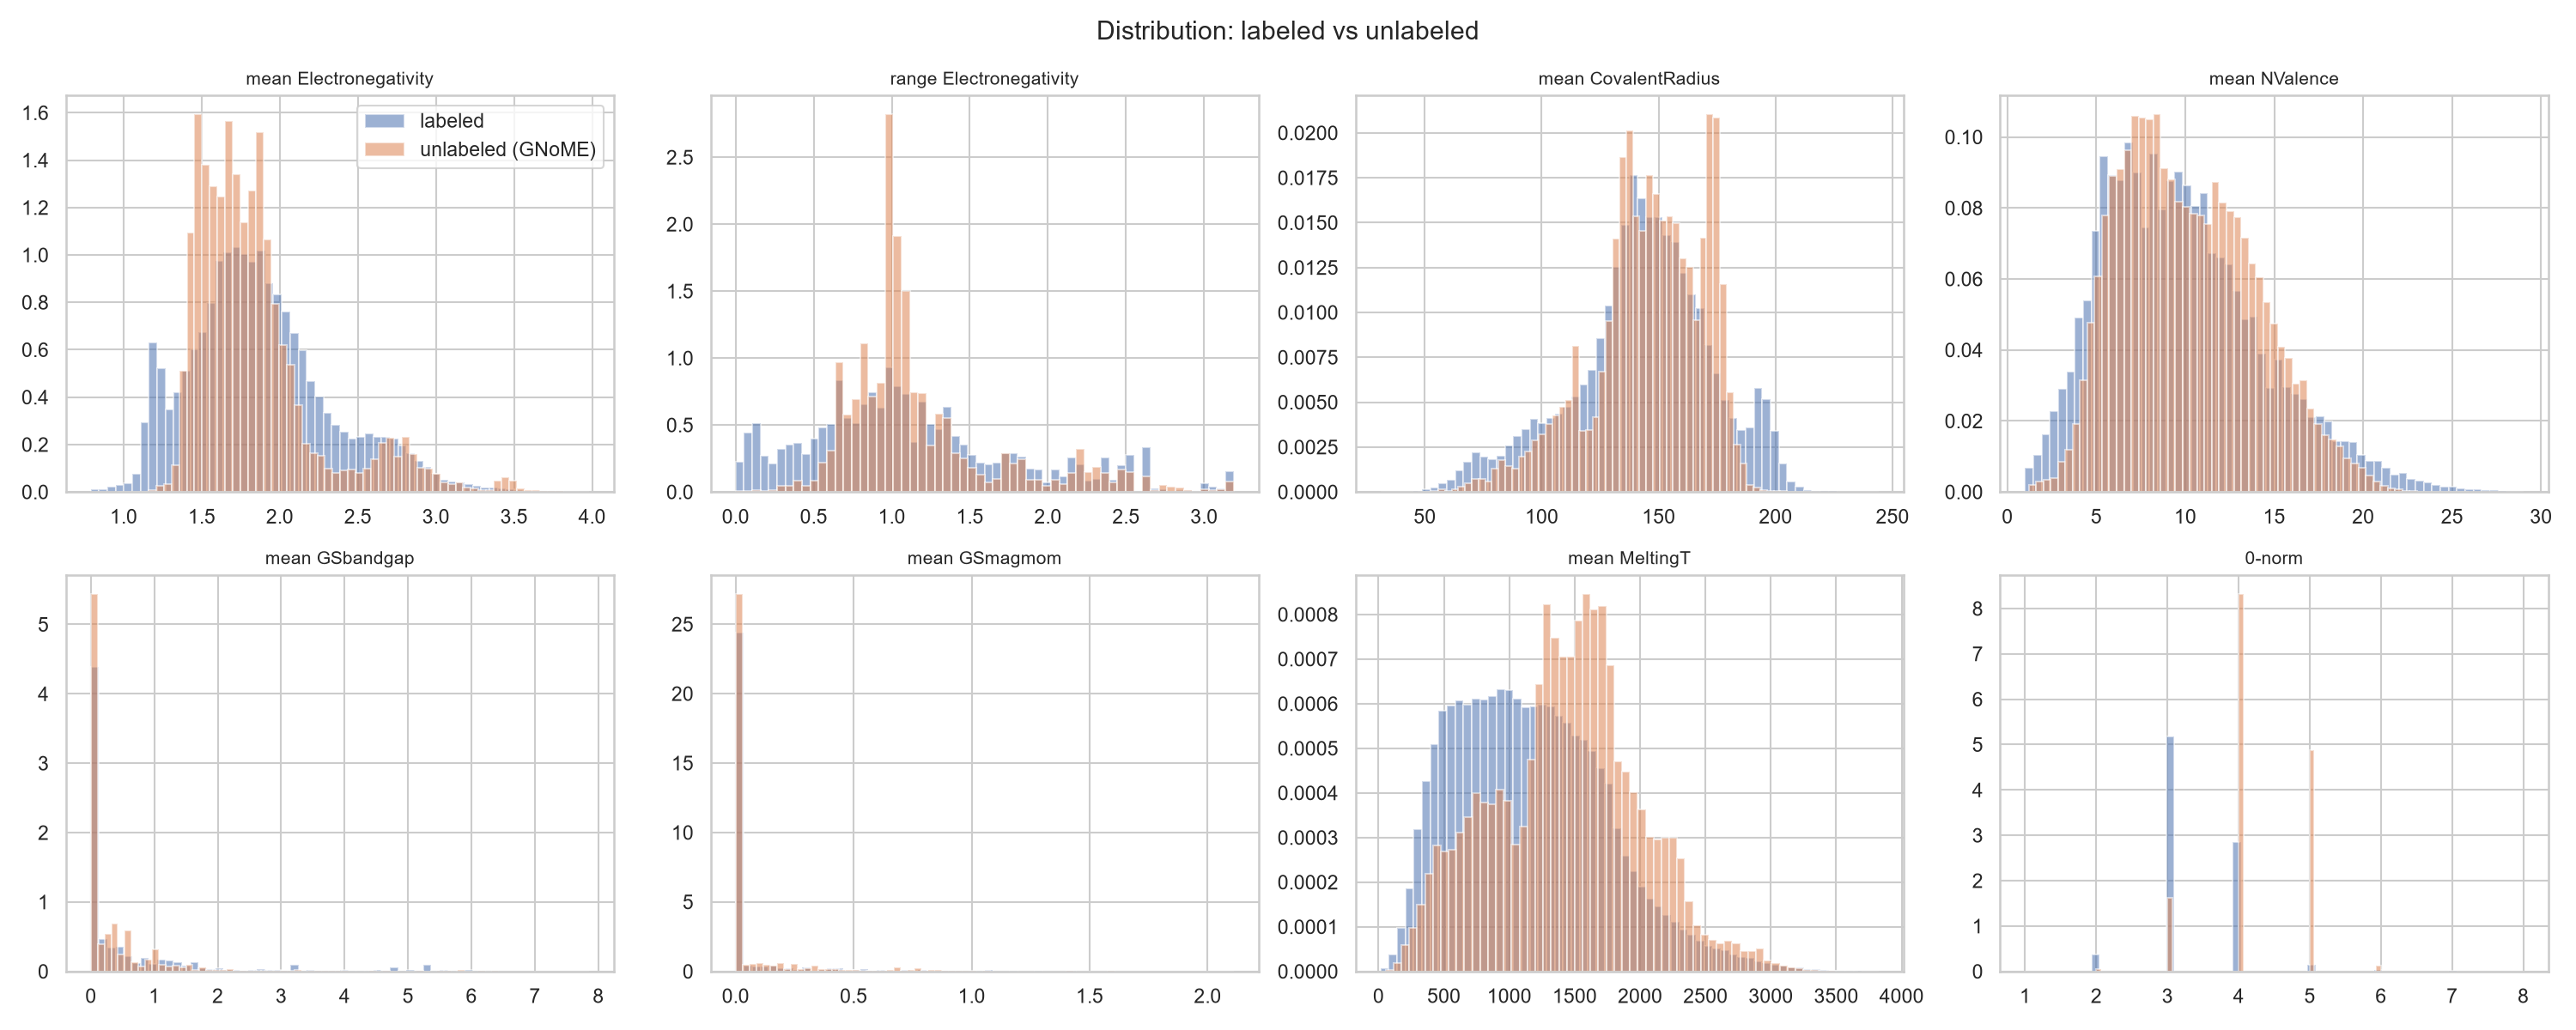
\includegraphics[width=\textwidth]{stability/labeled_vs_unlabeled.png}
  \caption{Distribution Labeled vs unlabeled}\label{fig:shift}
\end{figure}

The Kolmogorov--Smirnov tests confirm that labeled and unlabeled compositions are not drawn
from exactly the same distribution: for Alexandria most KS statistics stay below 0.25, whereas
for the Materials Project metallicity data they reach 0.43--0.48 (mean electronegativity,
melting temperature, number of elements). This distribution shift is an important factor in
the SSL results (Section~\ref{sec:discussion}).

\begin{figure}[H]
  \centering
  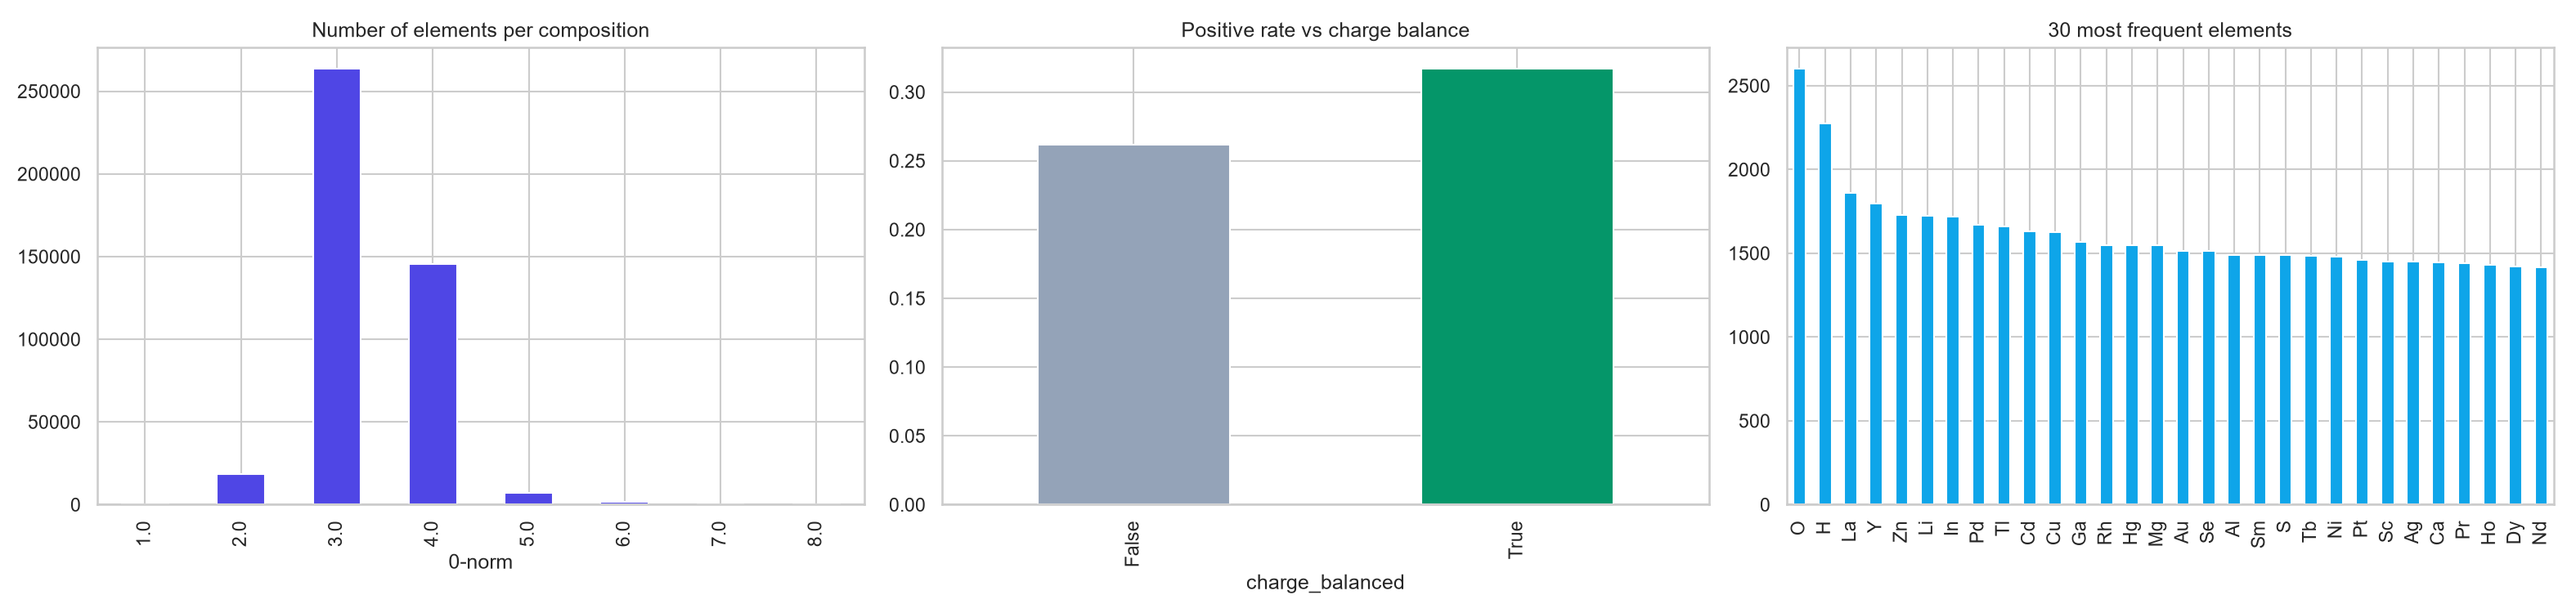
\includegraphics[width=\textwidth]{stability/chemical_rules.png}
  \caption{Chemical Rules}
\end{figure}

\begin{figure}[H]
  \centering
  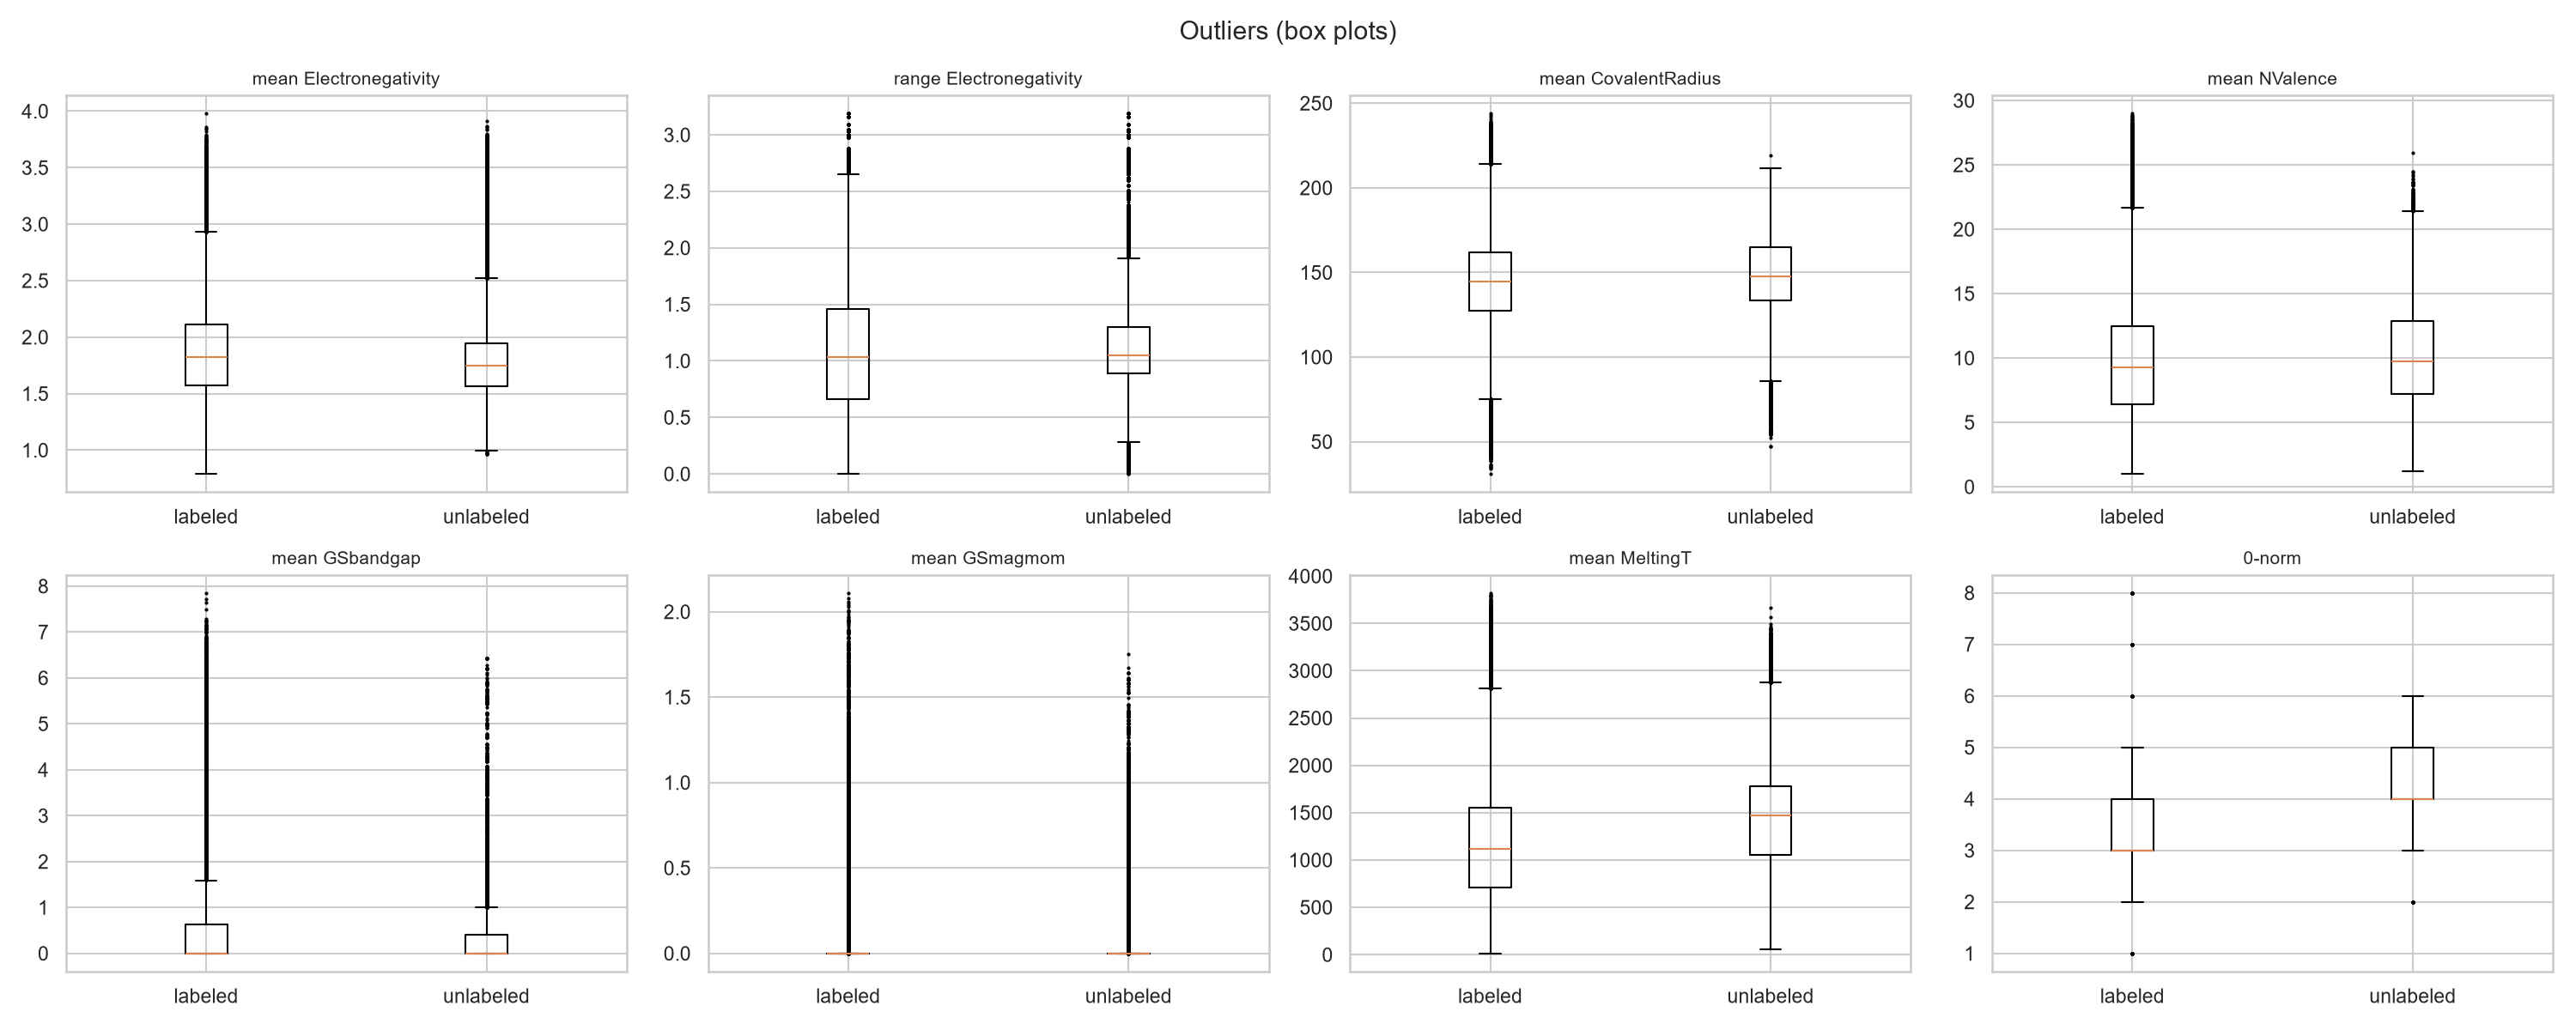
\includegraphics[width=\textwidth]{stability/outliers.png}
  \caption{Outliers}\label{fig:outliers}
\end{figure}

\item \textbf{Normalization and Scaling:} to ensure model stability, missing values are
imputed with the median, outliers are clipped at mean $\pm 3$ standard deviations (0.78\% of
the values for Alexandria, 0.95\% for Materials Project) and all features are standardized
with a \texttt{StandardScaler}. The preprocessing object is fitted on the training data only
and saved to ensure consistent transformation during inference.

\begin{figure}[H]
  \centering
  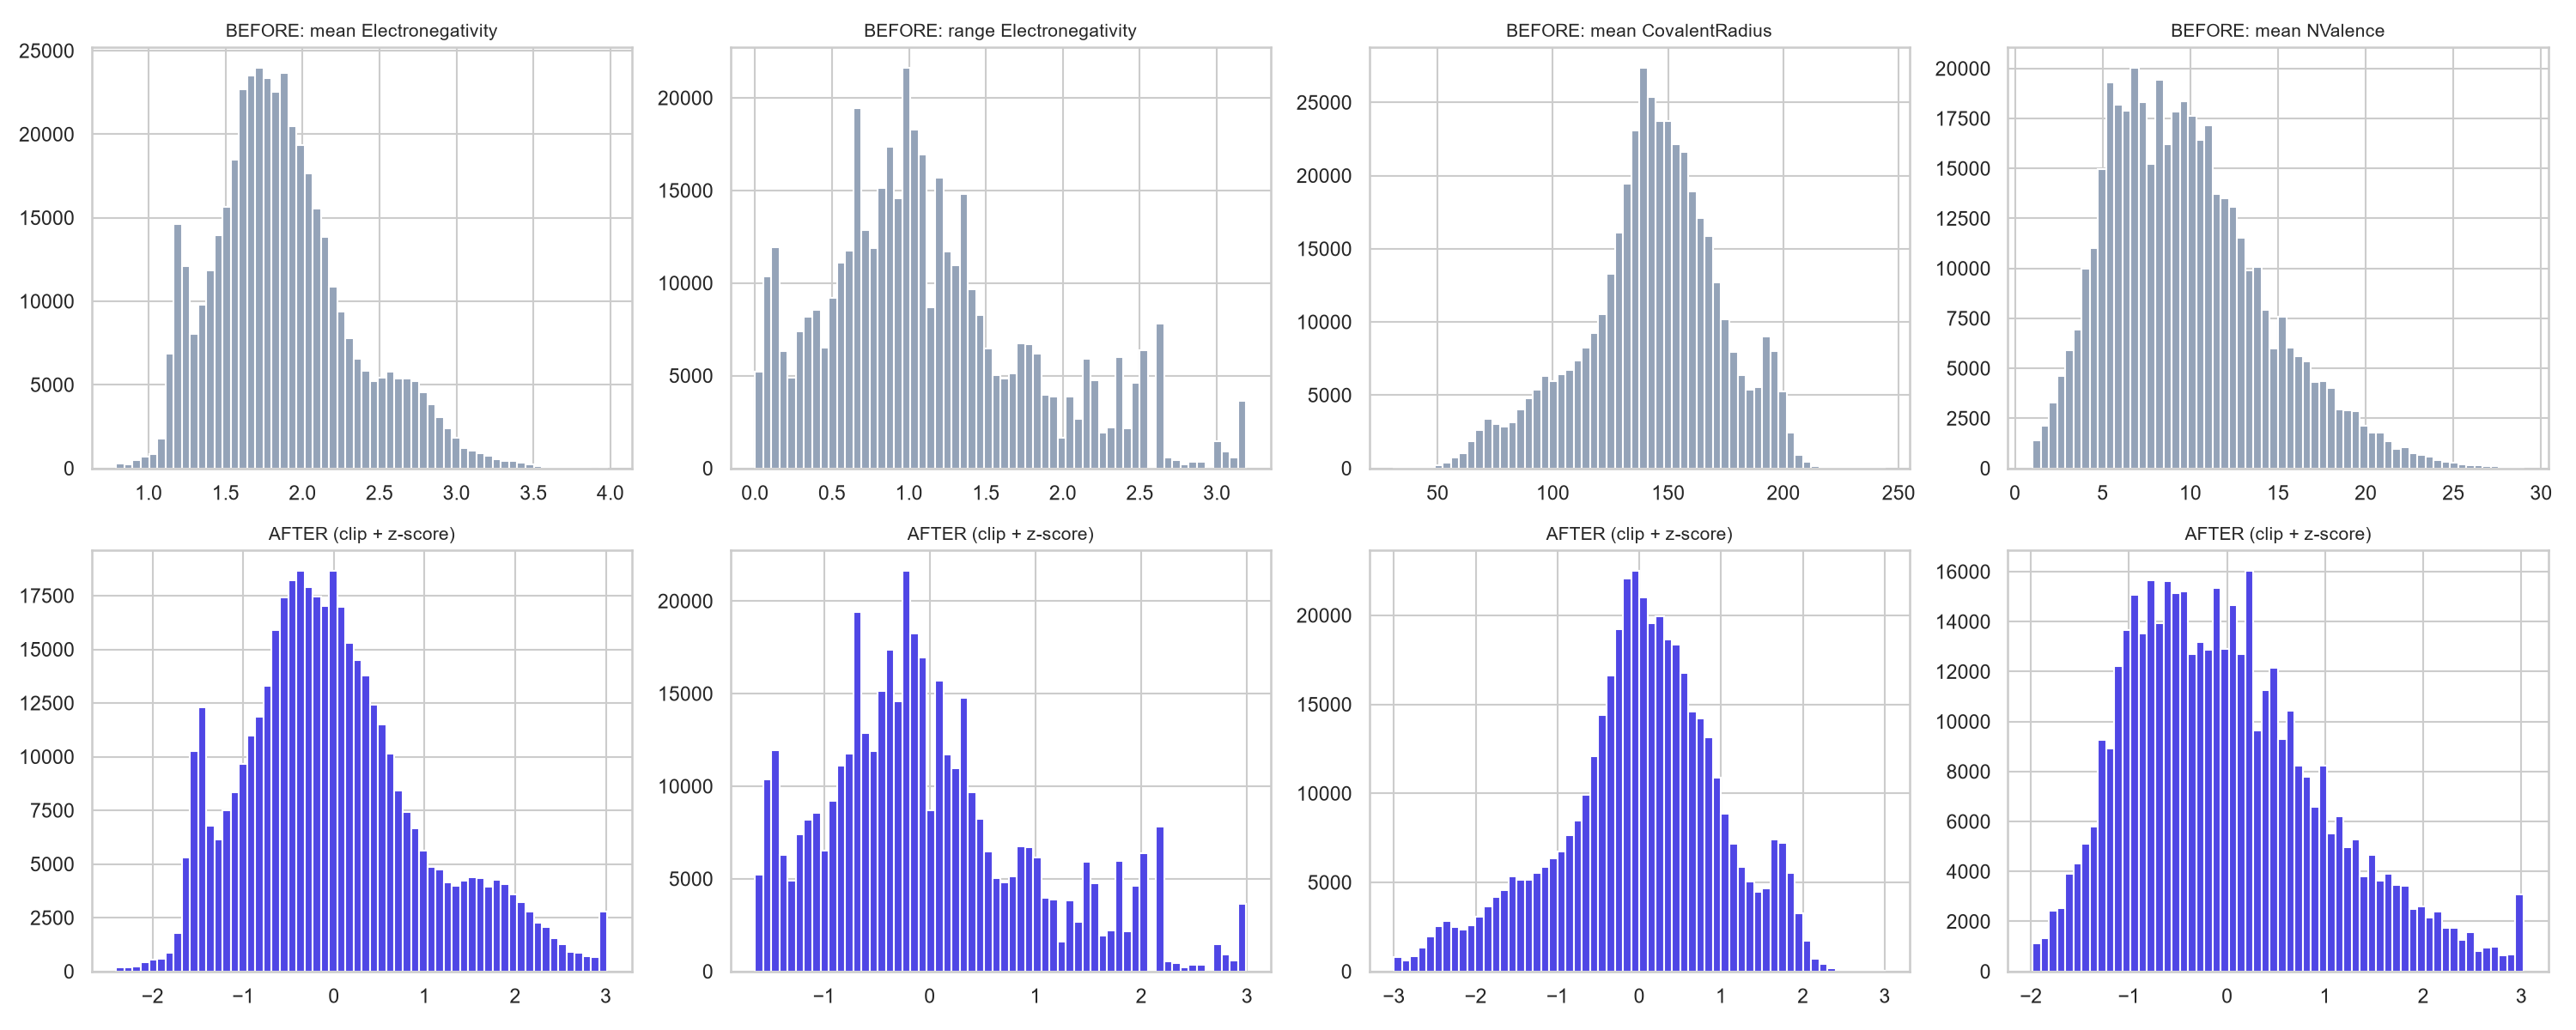
\includegraphics[width=\textwidth]{stability/normalization_before_after.png}
  \caption{Normalization of feature vectors (before and after clipping and z-scoring).}
\end{figure}

\item \textbf{Final Dataset Compilation:} the pipeline concludes by saving the processed
labeled and unlabeled datasets, ready for training. The output confirms the count of labeled
compositions, unlabeled compositions, and total features.

\begin{figure}[H]
\begin{console}
FINAL OUTPUT OF THE PREPROCESSING PIPELINE\\
==========================================================\\
metallicity : \MetalN{} labeled | 554,047 unlabeled (GNoME) | 142 descriptors | pos. rate \MetalPos{}\%\\
magnetism~~~: \MagN{} labeled | GNoME pool deduplicated | 142 descriptors | pos. rate \MagPos{}\%\\
stability~~~: \StabN{} labeled | 548,412 unlabeled (GNoME) | 142 descriptors | pos. rate \StabPos{}\%\\
band\_gap~~~~: \GapN{} labeled | 142 descriptors | pos. rate \GapPos{}\%\\
split: stratified 80/20 train/test, test set never used for training or tuning
\end{console}
\caption{Final output of the preprocessing pipeline showing dataset statistics.}
\end{figure}
\end{enumerate}

\clearpage
\section{Algorithmic Methods}\label{sec:methods}

In this project, we use five Semi-Supervised Learning (SSL) techniques. While all methods
leverage labeled and unlabeled data, their approach differs. Tree-ensemble classifiers (a
Random Forest reference and an Optuna-tuned LightGBM, written LightGBM$^*$) are used as the
\textbf{base model} for Self-Learning, Co-Training and Cluster-then-Label, while Label
Propagation and Label Spreading are graph-based methods operating directly on the
compositional-similarity graph. Every method is compared with a \textbf{supervised baseline}
trained on the same labeled samples only. The experimental protocol is identical for all
methods:

\begin{itemize}
  \item a stratified 80/20 train/test split; the test set (up to 20,000 evaluated
  compositions) is never used for training or tuning;
  \item a scarce \textbf{labeled budget of 1,000 compositions} drawn from the training set;
  \item unlabeled pools of \textbf{1,000, 5,000, 25,000 and 100,000} compositions, either from
  GNoME or from the training set with labels hidden;
  \item \textbf{3 random seeds} for every configuration, results reported as mean $\pm$ std;
  \item model selection with the \textbf{Composite Score = (F1 + ROC-AUC)/2}, which balances
  threshold-dependent (F1) and ranking (ROC-AUC) quality on imbalanced classes.
\end{itemize}

% ---------------------------------------------------------------------------- 5.1
\subsection{Self-Learning (Pseudo-Labeling)}

\subsubsection{Introduction}
Self-learning is an iterative SSL method where a tree-ensemble model trained on labeled data
predicts labels for unlabeled samples. High-confidence predictions are added to the labeled
set in successive iterations to refine performance.

\subsubsection{Theory}
Let $X_L$ and $y_L$ be the labeled data, and $X_U$ the unlabeled data. A model $f$ is trained
on $(X_L, y_L)$ and predicts $\hat{y}_U$ for $X_U$. Samples with prediction confidence above
threshold $\tau$ are added to the labeled set:
\[
X_L \leftarrow X_L \cup \{x \in X_U : \max f(x) \ge \tau\}, \qquad
y_L \leftarrow y_L \cup \{\hat{y}_U \text{ for selected } x\}
\]
This repeats until no new sample passes the threshold or the maximum number of iterations is
reached. We test $\tau \in \{0.75, 0.9\}$ with Random Forest and LightGBM$^*$ base learners.

\subsubsection{Workflow}
\begin{enumerate}
  \item Train the base model on labeled data.
  \item Predict labels for unlabeled samples.
  \item Add high-confidence predictions to the labeled set.
  \item Retrain the base model with the updated labeled set.
  \item Repeat until the stopping criteria.
\end{enumerate}

\begin{pycode}{Self-Learning with a tuned LightGBM base learner}
from sklearn.semi_supervised import SelfTrainingClassifier
from lightgbm import LGBMClassifier
import numpy as np

base = LGBMClassifier(**optuna_best_params, class_weight="balanced")   # tuned base model
self_training = SelfTrainingClassifier(base, threshold=0.9, max_iter=5)

# Combine labeled and unlabeled data (-1 = unlabeled)
X_combined = np.vstack([X_labeled, X_unlabeled])
y_combined = np.concatenate([y_labeled, -np.ones(len(X_unlabeled), dtype=int)])

self_training.fit(X_combined, y_combined)
y_pred_proba = self_training.predict_proba(X_test)[:, 1]
y_pred = (y_pred_proba >= 0.5).astype(int)
\end{pycode}

% ---------------------------------------------------------------------------- 5.2
\subsection{Co-Training (Multi-View Learning)}

\subsubsection{Introduction}
Co-training trains two models on different feature subsets (views). Each model predicts labels
for unlabeled samples to improve the other iteratively.

\subsubsection{Theory}
Let $(X^1, X^2)$ be two feature views and $f^1, f^2$ two classifiers trained on
$(X^1_L, y_L)$ and $(X^2_L, y_L)$. In our materials setting, \textbf{view~1} contains the
elemental-property statistics (electronegativity, radius, melting point, Mendeleev number,
\dots) and \textbf{view~2} the stoichiometry, valence-orbital and valence-electron descriptors.
Each classifier labels the unlabeled samples it is most confident about (probability above
$\tau=0.85$, keeping the labeled class ratio), and these pseudo-labels are added to the shared
labeled set. The final prediction averages the probabilities of both views:
$p(x) = \tfrac{1}{2}\big(f^1(x^1) + f^2(x^2)\big)$.

\subsubsection{Workflow}
\begin{enumerate}
  \item Split features into two views.
  \item Train a model on each view with labeled data.
  \item Predict labels for unlabeled data in each view.
  \item Add high-confidence predictions to the labeled set used by the other view.
  \item Retrain and repeat (5--8 rounds).
\end{enumerate}

\begin{pycode}{Co-Training Example (pipeline/ssl\_core.py)}
for round in range(n_rounds):
    c1 = clone(base).fit(XL[:, view1], yL)      # elemental-property view
    c2 = clone(base).fit(XL[:, view2], yL)      # stoichiometry / valence view
    for clf, view in ((c1, view1), (c2, view2)):
        p = clf.predict_proba(X_unl[pool][:, view])[:, 1]
        for cls, prob in ((1, p), (0, 1 - p)):
            quota = round(per_round * (pos_ratio if cls == 1 else 1 - pos_ratio))
            cand = np.where(prob >= threshold)[0]                 # confident samples
            cand = cand[np.argsort(-prob[cand])][:quota]
            add_idx.extend(pool[cand]); add_lab.extend([cls] * len(cand))
    XL = np.vstack([XL, X_unl[add_idx]]); yL = np.concatenate([yL, add_lab])
    pool = np.setdiff1d(pool, add_idx)
proba = (c1.predict_proba(X[:, view1]) + c2.predict_proba(X[:, view2])) / 2
\end{pycode}

% ---------------------------------------------------------------------------- 5.3
\subsection{Label Propagation}

\subsubsection{Introduction}
Label Propagation is a graph-based SSL method. Nodes represent materials, and edges encode
compositional similarity. Labels from labeled nodes propagate iteratively to unlabeled nodes.

\subsubsection{Theory}
Construct a similarity graph $G = (V, E)$ with adjacency matrix $W$ (RBF kernel
$W_{ij}=\exp(-\gamma\|x_i-x_j\|^2)$ for pools up to 10,000 nodes, sparse $k$-nearest-neighbour
graph with $k=10$ for larger pools). Let $Y$ be the label matrix with labeled nodes initialized
to their class. Labels are propagated iteratively:
\[
Y^{(t+1)} = \alpha W Y^{(t)} + (1-\alpha) Y^{(0)}
\]
where $\alpha \in (0,1)$ controls the influence of neighbours (Label Propagation clamps the
labeled nodes, i.e.\ hard labels). Because graph methods tend to drift towards the majority
class on imbalanced data, we apply \textbf{class mass normalization} (Zhu et al., 2003): the
class scores are rescaled so that the class proportions predicted on the unlabeled nodes match
the class prior estimated from the labeled nodes.

\subsubsection{Workflow}
\begin{enumerate}
  \item Build the similarity graph from the standardized descriptors.
  \item Initialize the label matrix $Y^{(0)}$ (labeled nodes only).
  \item Propagate labels iteratively until convergence.
  \item Apply class mass normalization and assign labels to unlabeled and test nodes.
\end{enumerate}

\begin{pycode}{Label Propagation - Core Step}
from sklearn.semi_supervised import LabelPropagation

X_combined = np.vstack([X_labeled, X_unlabeled])
y_combined = np.concatenate([y_labeled, np.full(len(X_unlabeled), -1)])

lp = LabelPropagation(kernel="knn", n_neighbors=10, max_iter=1000, n_jobs=-1)
lp.fit(X_combined, y_combined)

# class mass normalization: predicted class proportions = labeled class prior
model = ClassMassNormalized(lp, n_labeled=len(y_labeled), prior_pos=y_labeled.mean(),
                            X_u=X_unlabeled)
y_pred_proba = model.predict_proba(X_test)[:, 1]
\end{pycode}

% ---------------------------------------------------------------------------- 5.4
\subsection{Label Spreading}

\subsubsection{Introduction}
Label Spreading extends Label Propagation by normalizing the adjacency matrix, smoothing label
assignments, and reducing sensitivity to noisy edges. Labeled nodes are allowed to change
(soft labels).

\subsubsection{Theory}
Normalized adjacency matrix:
\[
S = D^{-1/2} W D^{-1/2}, \qquad Y^{(t+1)} = \alpha S Y^{(t)} + (1-\alpha) Y^{(0)}
\]
where $D$ is the degree matrix. We test $\alpha \in \{0.2, 0.8\}$ and also build the graph in
the 32-dimensional \textbf{self-supervised embedding} (Section~5.6.3) instead of the raw
descriptor space.

\subsubsection{Workflow}
\begin{enumerate}
  \item Build the similarity graph and normalize the adjacency matrix.
  \item Initialize the label matrix $Y^{(0)}$ with the labeled nodes.
  \item Iteratively propagate and smooth labels.
  \item Assign labels after convergence (with class mass normalization).
\end{enumerate}

\begin{pycode}{Label Spreading - Core Step}
from sklearn.semi_supervised import LabelSpreading

ls = LabelSpreading(kernel="knn", n_neighbors=10, alpha=0.2, max_iter=1000, n_jobs=-1)
ls.fit(X_combined, y_combined)
model = ClassMassNormalized(ls, len(y_labeled), y_labeled.mean(), X_u=X_unlabeled)
y_pred_proba = model.predict_proba(X_test)[:, 1]
\end{pycode}

% ---------------------------------------------------------------------------- 5.5
\subsection{Traditional Materials Informatics for Photovoltaic Band Gap}

For photovoltaic band-gap classification, we implemented a classical materials-informatics
pipeline with genetic-algorithm optimization. The task is to recognize compositions whose PBE
band gap lies in the photovoltaic window $1.1 \le E_g \le 1.7$\,eV (\GapN{} Materials Project
compositions, \GapPos{}\% positives).

\subsubsection{Feature Generation and Optimization}
The 142 Magpie/stoichiometry descriptors were generated for every composition. Seven
classifiers (Random Forest, Extra Trees, XGBoost, LightGBM, Logistic Regression, $k$-NN and an
RBF Support Vector Machine) were compared, and a DEAP-based genetic algorithm optimized the
descriptor subset by maximizing the cross-validated ROC-AUC.

\subsubsection{Applicability Domain Assessment}
Following OECD guidelines, we implemented an applicability-domain framework using PCA
projection, K-Means clustering, and distance-based thresholds to flag predictions with low
confidence. The same check is exposed by the web application for every user query.

\subsubsection{Theoretical Foundations}

\textbf{Genetic Algorithms in Feature Selection:} genetic algorithms (GAs) are
population-based optimization techniques inspired by natural selection~\cite{deap}. For feature
selection, each individual is a binary vector indicating descriptor inclusion/exclusion. The
algorithm evolves through tournament selection, two-point crossover and bit-flip mutation:
\[
\text{Fitness} = \text{ROC-AUC} - \lambda \cdot \frac{\#\text{selected features}}{\#\text{total features}}
\]
where $\lambda = 0.05$ controls the penalty for feature count. The GA explores the feature
space combinatorially, making it particularly suitable for high-dimensional descriptor
selection in materials informatics.

\textbf{Applicability Domain Theory:} the applicability domain (AD) defines the chemical space
where a model provides reliable predictions~\cite{oecd}. Multiple approaches were employed:
\begin{itemize}
  \item \textbf{Distance-Based AD:} the mean Euclidean distance $D_i$ of composition $i$ to its
  five nearest training compositions (in the GA-selected, standardized descriptor space) is
  compared with the 95th percentile of the same distance over the training set:
  \[
  D_i = \frac{1}{5}\sum_{j \in \mathrm{kNN}(i)} \lVert x_i - x_j \rVert_2, \qquad
  i \in \text{AD} \iff D_i \le P_{95}\big(D_{\text{train}}\big)
  \]
  \item \textbf{PCA-Based AD:} test compositions projecting outside the region occupied by the
  training compositions in PCA space are flagged as outliers.
  \item \textbf{Cluster-Based AD:} test compositions assigned to sparsely populated training
  clusters (K-Means, $k = 6$) are considered at the border of the AD.
\end{itemize}

\textbf{Performance Metrics:} model performance was evaluated using the receiver operating
characteristic area under the curve (ROC-AUC), which measures the trade-off between true
positive rate (sensitivity) and false positive rate (1-specificity):
\[
\text{ROC-AUC} = \int_0^1 \text{TPR}\big(\text{FPR}^{-1}(x)\big)\,dx
\]
ROC-AUC values range from 0.5 (random performance) to 1.0 (perfect discrimination), with values
above 0.8 generally considered good and above 0.9 excellent. Because the positive class is
rare (\GapPos{}\%), we also report the precision--recall AUC (PR-AUC, random level =
\GapPos{}\%) and the F1-score.

% ---------------------------------------------------------------------------- 5.6
\subsection{Unsupervised and Self-Supervised Components}

\subsubsection{Cluster-then-Label}
K-Means ($k=100$, unsupervised) is run on the union of labeled and unlabeled compositions. For
every cluster containing at least three labeled compositions whose labels are at least 80\%
pure, the unlabeled members receive the majority label. The base learner is then trained on
labeled plus pseudo-labeled compositions, pseudo-labels being weighted by 0.5.

\subsubsection{Association-Rule Mining (Apriori)}
Each composition is treated as a \emph{transaction} whose items are its chemical elements,
extended with the property item (\texttt{STABLE}, \texttt{MAGNETIC}, \texttt{METAL},
\texttt{PV\_GAP}) used only as a rule consequent. The Apriori algorithm extracts frequent
itemsets and rules $A \Rightarrow B$ scored by
\[
\text{supp}(A\Rightarrow B) = P(A \cup B),\quad
\text{conf}(A\Rightarrow B) = \frac{P(A \cup B)}{P(A)},\quad
\text{lift}(A\Rightarrow B) = \frac{\text{conf}(A\Rightarrow B)}{P(B)}
\]
A lift above 1 means that the elements of $A$ make property $B$ more likely than average. The
same mining on GNoME alone (no property item) reveals which elements co-occur in new materials.

\subsubsection{Self-Supervised Pre-training (Masked Autoencoder)}
The pretext task requires no labels: 25\% of the 142 descriptors of each GNoME composition are
masked (set to the mean) and an MLP autoencoder
($142 \rightarrow 128 \rightarrow 32 \rightarrow 128 \rightarrow 142$, tanh) learns to
reconstruct the complete, clean vector from the 554,054 unlabeled compositions. The
32-dimensional bottleneck is a learned \emph{materials embedding}; downstream classifiers are
trained on it (alone or concatenated with the raw descriptors), and Label Spreading is also run
on a graph built in this embedding space.

\begin{pycode}{Masked-feature autoencoder (pipeline/self\_supervised.py)}
net = MLPRegressor(hidden_layer_sizes=(128, 32, 128), activation="tanh", batch_size=512)
for epoch in range(20):
    mask = rng.random(Z_train.shape) < 0.25          # mask 25 % of the descriptors
    net.partial_fit(np.where(mask, 0.0, Z_train), Z_train)   # reconstruct clean vector
embedding = encode(X)                                   # 32-d bottleneck layer
\end{pycode}

\clearpage
\section{Results Comparison on Metallicity}

The metallicity task (Materials Project, \MetalN{} compositions, \MetalPos{}\% metals) was
trained with 1,000 labeled compositions and five semi-supervised methods, the masked-autoencoder
features and nine supervised baselines (\MetalInRuns{} models per unlabeled pool). Every score
is the mean over 3 seeds on the same \MetalInNTest{} held-out test compositions.

\subsection*{Comparison of SSL Methods}

\resfig{\textwidth}{results/metallicity/indist/metallicity_methods_comparison_balanced.png}{Comparison
of SSL methods on the Metallicity dataset (unlabeled pool: same database, labels hidden).}

\maybeinput{table_metallicity_indist}
\maybeinput{table_metallicity_gnome}

With the unlabeled compositions taken from the same database, \MetalInBestMethod{}
(\texttt{\MetalInBestConfig}) reaches a composite score of \MetalInBestComp{}, against
\MetalInBaseComp{} for the Optuna-tuned \MetalInBaseConfig{} baseline (\MetalInImpr\%).
Self-Training, Cluster-then-Label and the self-supervised features are statistically tied with
the baseline (differences below one standard deviation). The graph methods (Label Propagation
and Label Spreading) are clearly behind (composite $\approx 0.85$): the $k$-NN graph built on
142 descriptors does not separate metals from insulators as well as a boosted tree does.

With GNoME as the unlabeled pool, no SSL method beats the baseline: the best one,
\MetalGnBestSSL{}, reaches \MetalGnBestSSLComp{} (\MetalGnImpr\%), and the graph methods fall
to 0.75--0.79. GNoME compositions follow a different distribution (Figure~\ref{fig:shift}), so the labels
that are propagated or pseudo-labelled on them are less reliable.

\subsection*{Effect of the Number of Unlabeled Compositions}

\resfig{\textwidth}{results/metallicity/indist/metallicity_learning_curves.png}{Composite score
and F1-score versus the number of unlabeled compositions (metallicity, same-database pool).}

\maybeinput{poolsize_metallicity_indist}
\maybeinput{poolsize_metallicity_gnome}

Adding more unlabeled compositions does \emph{not} help: every method is best with the
smallest pool (1,000 unlabeled) and degrades steadily up to the largest one (60,945
for the same database, 100,000 for GNoME). Self-Training is the most
robust, because its 0.9 confidence threshold only accepts pseudo-labels the model is sure
about. The graph methods degrade fastest, because each additional unlabeled node also spreads
errors.

\subsection*{Label Budget and Supervised Model Zoo}

\resfig{0.8\textwidth}{results/metallicity/indist/metallicity_label_budget_curve.png}{Label-budget
curve for metallicity: best supervised baseline versus best SSL configuration.}

\maybeinput{budget_metallicity_indist}
\maybeinput{zoo_metallicity_indist}

Labels matter much more than unlabeled data: going from 1,000 to 5,000 labels raises the
composite from about 0.87 to 0.90, while using all \MetalN{} compositions brings the fully
supervised model to \MetalInFullComp{} (ROC-AUC \MetalInFullAUC{}). The SSL and baseline curves
overlap at every budget (differences of at most 0.001). Among supervised
models, gradient boosting (LightGBM, XGBoost) and Random Forest are equivalent; linear, $k$-NN
and MLP models are about 0.02 lower.

\subsection*{Selected Model}

The deployed model keeps the architecture selected at 1,000 labels and is re-trained on all
training labels plus the unlabeled pool. On the held-out test set it reaches a composite score
of \MetalSelComp{} (ROC-AUC \MetalSelAUC{}, F1 \MetalSelFone{}, accuracy \MetalSelAcc{}).

Consequently, \textbf{\MetalSelMethod{}} (\texttt{\MetalSelConfig}) is selected as the primary
architecture for the deployment phase of the metallicity prediction module.

\clearpage
\section{Results Comparison on Magnetism}

(Results are being computed.)

\clearpage
\section{Results Comparison on Stability}

(Results are being computed.)

\clearpage
\section{Discussion and Limitations}\label{sec:discussion}

The results show that the performance gains achieved using SSL are not always significant
(Table~\ref{tab:ssl-overview}). With 1,000 labels, the best semi-supervised method beats the
Optuna-tuned supervised baseline by at most \MagInImpr\% (magnetism, Self-Training). On
metallicity and stability the gain is within one standard deviation, and with the GNoME pool
on metallicity no SSL method beats the baseline at all. This suggests that SSL is not a
universal solution and that its effectiveness depends on data distribution and underlying
assumptions:
\begin{itemize}
  \item \textbf{Strong baselines.} Gradient-boosted trees trained on 142 Magpie descriptors
  already capture most of what 1,000 labels can teach. The label-budget curves show that SSL
  helps most at 250--500 labels and that the gap closes after 2,500 labels.
  \item \textbf{Distribution shift.} The KS statistics between labeled and GNoME compositions
  reach 0.48 (Figure~\ref{fig:shift}). Unlabeled data from a different distribution violate the
  cluster and manifold assumptions, which is why the GNoME pool is never better than the
  same-database pool for the graph methods.
  \item \textbf{More unlabeled data is not better.} For almost every method the composite
  score decreases from 1,000 to 100,000 unlabeled compositions: errors in the pseudo-labels
  accumulate faster than useful information. Only Self-Training with a high confidence
  threshold (0.9) is robust to the pool size.
  \item \textbf{Graph methods do not scale to this feature space.} Label Propagation and
  Label Spreading are always last, even after class-mass normalization. Euclidean neighbours in
  descriptor space do not share labels reliably, and an exact RBF graph is only possible for
  the smallest pools.
  \item \textbf{Composition-only descriptors.} Stability (\StabSelComp{} composite even after
  deployment) depends on the crystal structure and on competing phases, which a composition
  cannot encode. Structure-aware graph neural networks (CGCNN, MEGNet, ALIGNN) would be needed
  for a large gain.
  \item \textbf{DFT labels.} All labels come from PBE calculations. PBE underestimates band
  gaps by 30--50\% on average, so the 1.1--1.7\,eV photovoltaic window is a window on
  \emph{PBE} gaps, and real absorbers may fall slightly outside it.
\end{itemize}

The self-supervised masked autoencoder learns a good representation (R$^2$ = \AERtwo{} on all
descriptors, \AERtwoMasked{} on the hidden ones). As extra features it is tied with the raw
descriptors on metallicity and slightly below them on magnetism and stability, but it gives a compact 32-dimensional space for the nearest-material search of
the application. The unsupervised analysis (Apriori rules, K-Means) gives interpretable
chemistry, for example \{Fe\} $\Rightarrow$ MAGNETIC with a lift of 3.4, and helps explain the
models, but it does not replace a classifier.

The traditional materials-informatics approach for the photovoltaic band gap demonstrated
that, for a well-defined target, classical methods with feature optimization provide strong
performance with interpretability. The genetic algorithm successfully identified \GAFinalN{}
key descriptors from an initial set of 142 (a 63\% reduction) with a test ROC-AUC of
\GapGAAUC{} against \GapAllAUC{} for all descriptors, and the applicability domain covers
\ADFracIn\% of the test compositions.

Alternative approaches such as Active Learning, Transfer Learning, or deep representations of
materials may provide better results in certain scenarios. Since our models are cheap to
evaluate and the GNoME pool is huge, the most promising next step is a semi-supervised
\emph{active-learning} loop (Figure~\ref{fig:al}): instead of labelling random compositions,
the model chooses the most informative or most promising candidates, these are computed by
DFT, and the model is re-trained.

\begin{figure}[H]
  \centering
  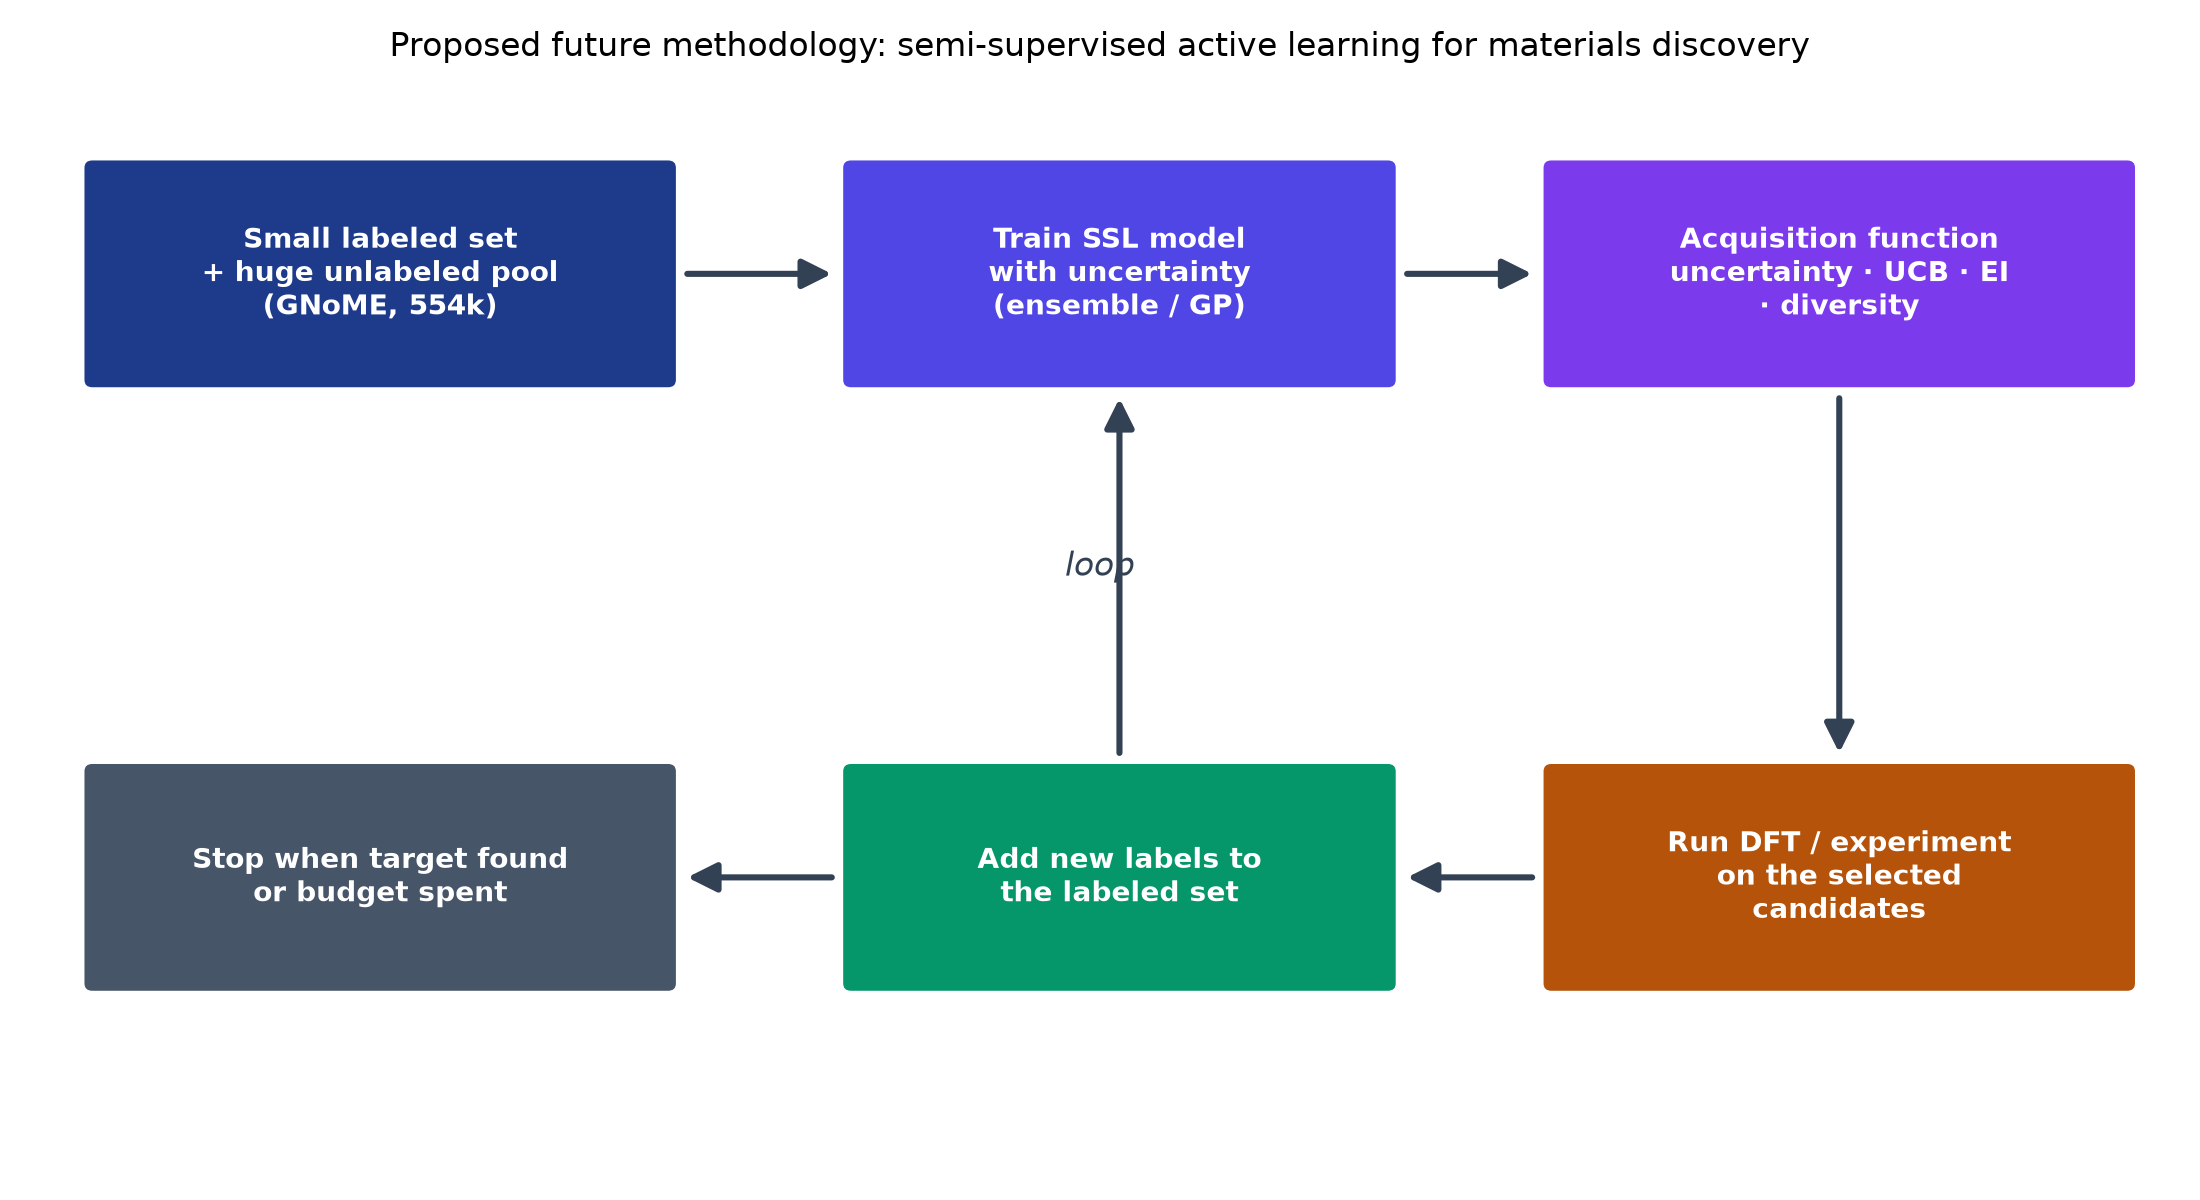
\includegraphics[width=\textwidth]{schematics/active_learning_loop.png}
  \caption{Better methodology for future: semi-supervised active learning.}\label{fig:al}
\end{figure}

\clearpage
\section{Technologies Used}

\newcommand{\techitem}[3]{%
  \subsection{#1}
  \begin{minipage}[c]{0.70\textwidth}#2\end{minipage}\hfill
  \begin{minipage}[c]{0.24\textwidth}\centering\includegraphics[width=0.85\linewidth]{logos/#3}\end{minipage}
  \vspace{1.2em}}

\techitem{Docker}{Docker is a containerization platform that allows packaging an application
and its dependencies into a lightweight, portable container. A multi-stage Dockerfile builds
the React frontend and the Python API into a single image, which standardizes the development
environment and simplifies the deployment of the API and web application.}{docker.png}

\techitem{React}{React is an open-source JavaScript library developed by Meta, used to create
interactive user interfaces. It was used (with Vite) to develop the \textbf{Frontend} of our
application, providing a smooth and responsive user experience for composition input,
3D crystal visualization (3Dmol.js) and prediction display.}{react.png}

\techitem{FastAPI}{FastAPI is a modern and high-performance web framework for building APIs
with Python. It was chosen as the \textbf{Backend} to serve our Machine Learning models due to
its speed, native asynchronous support, and automatic documentation generation.}{fastapi.png}

\techitem{Jupyter Notebook}{Jupyter Notebook is an open-source web application for creating
and sharing documents containing code, equations, and visualizations. It served as the main
tool for data enhancement, Exploratory Data Analysis (EDA), preprocessing, and the
presentation of the SSL experiments.}{jupyter.png}

\techitem{GitHub}{GitHub is a Git-based source code management platform. It was used for
project hosting, team collaboration, continuous integration (GitHub Actions: linting and
tests) and version control of the source code.}{github.png}

\techitem{pymatgen \& matminer}{pymatgen and matminer are the reference open-source Python
libraries of materials informatics. They were essential for parsing chemical formulas,
handling compositions and crystal structures, downloading the Matbench datasets and defining
the Magpie descriptors needed for the models.}{pymatgen.png}

\subsection{scikit-learn, LightGBM and Optuna}
scikit-learn provides the semi-supervised algorithms (Self-Training, Label Propagation, Label
Spreading), the classical models and the evaluation metrics; LightGBM and XGBoost provide fast
gradient-boosting learners, and Optuna performs the Bayesian (TPE) hyper-parameter search used
to tune the base learners. DEAP implements the genetic algorithm and mlxtend the Apriori
association-rule mining.

\clearpage
\section{Frontend Interface}

To demonstrate practical applicability, a web application was developed with React (frontend)
and FastAPI (backend). The backend exposes the deployed models through a REST API
(\texttt{/materials/predict}, \texttt{/materials/analyze}, \texttt{/materials/structure},
\texttt{/materials/models-info}), while the frontend allows users to build a chemical
composition, inspect its crystal structure and receive stability, magnetism, metallicity and
photovoltaic band-gap predictions. The application is packaged in a single Docker image in which
FastAPI also serves the compiled React interface.

\begin{figure}[H]
  \centering
  \safeimg{\textwidth}{screenshots/01_start.png}
  \caption{Starting Interface}
\end{figure}

\begin{figure}[H]
  \centering
  \safeimg{\textwidth}{screenshots/02_editor.png}
  \caption{Composition editor Interface (periodic table)}
\end{figure}

\begin{figure}[H]
  \centering
  \safeimg{\textwidth}{screenshots/03_input.png}
  \caption{Inputing formula Interface}
\end{figure}

\begin{figure}[H]
  \centering
  \safeimg{\textwidth}{screenshots/04_viewer.png}
  \caption{3D crystal View Interface}
\end{figure}

\begin{figure}[H]
  \centering
  \safeimg{\textwidth}{screenshots/05_analyze.png}
  \caption{Analyze Material Interface}
\end{figure}

\begin{figure}[H]
  \centering
  \safeimg{\textwidth}{screenshots/06_results.png}
  \caption{Results Interface}
\end{figure}

\clearpage
\section{Conclusion}

(Results are being computed.)


\end{document}
